\documentclass[8pt,a4paper]{scrartcl}

\usepackage[english]{babel}

\input{../Headerfiles/Packages}
\input{../Headerfiles/Titles}
\input{../Headerfiles/Commands}
\input{../Headerfiles/ENVIRONMENTS}
\graphicspath{{Pictures/}}
\parindent 0pt

\title{Introduction to Machine Learning}
\author{GianAndrea Müller}

\newtheorem{theorem}{Theorem}
\newtheorem{define}{Definition}
\newcommand{\Argmin}[2]{\text{arg}\underset{#1}{\min}\left(#2\right)}
\newcommand{\Argmax}[2]{\text{arg}\underset{#1}{\max}\left(#2\right)}

\begin{document}
\begin{multicols*}{3}
\maketitle
\tableofcontents
\end{multicols*}

\begin{multicols*}{3}

\section*{Maths}

\subsection*{Probability}

\subsubsection*{Most Important Distributions}

\small
\mportabflex{lllll}{
Verteilung&$p(x)$&$W_X$&$\expe{X}$&$\var{X}$\\
\hline
Bernoulli(p)&$p^x(1-p)^{1-x}$&$\{0,1\}$&$p$&$p(1-p)$\\
Bin(n,p)&${n\choose k}p^x(1-p)^{n-x}$&$\{0,\ldots,n\}$&$np$&$np(1-p)$\\
Mul(n,k,$p_i$)&$\frac{n!}{\prod_{i=0}^k x_i!}\prod\limits_{i=0}^k p_i^{x_i}$&&$n p_i$&$np_i(1-p_i)$\\
Geom(p)&$p(1-p)^{x-1}$&$\{1,2,\ldots\}$&$\frac{1}{p}$&$\frac{1-p}{p^2}$\\
Pois($\lambda$)&$e^{-\lambda}\frac{\lambda^x}{x!}$&$\{0,1,\ldots\}$&$\lambda$&$\lambda$\\
Uni(a,b)&$\frac{1}{b-a}$&$[a,b]$&$\frac{a+b}{2}$&$\frac{(b-a)^2}{12}$\\
Exp($\lambda$)&$\lambda e^{-\lambda x}$&$\mathbb{R}_+$&$\frac{1}{\lambda}$&$\frac{1}{\lambda^2}$\\
Gamma($\alpha,\lambda$)&$\frac{\lambda^\alpha}{\Gamma(\alpha)}x^{\alpha-1}e^{-\lambda x}$&$\mathbb{R}_+$&$\frac{\alpha}{\lambda}$&$\frac{\alpha}{\lambda^2}$\\
$\mathcal{N}(x;\mu,\sigma^2)$&$\frac{1}{\sqrt{2\pi}\sigma}e^{-\onha(\frac{x-\mu}{\sigma})^2}$&$\mathbb{R}$&$\mu$&$\sigma^2$\\
\hline
}
\normalsize

\mportant{$\mathcal{N}_k(\vec{x};\vec{\mu},\Sigma)=\frac{\text{exp}\left(-\frac{1}{2}(\vec{x}-\vec{\mu})^T\Sigma^{-1}(\vec{x}-\vec{\mu})\right)}{(2\pi)^k\sqrt{\det(\Sigma)}}$\\}

\mportant{$\ln(\mathcal{N}_k)=-\frac{k}{2}\ln(2\pi)-\frac{1}{@}\ln(|\Sigma|)-\frac{1}{2}(x-\mu)^T\Sigma^{-1}(x-\mu)$}

\paragraph{Beta Priors}

\mportant{$\text{Beta}(\theta,\alpha_+,\alpha_-)=\frac{1}{B(\alpha_+,\alpha_-)}\theta^{\alpha_+-1}(1-\theta)^{\alpha_--1}$}

where $B(\alpha_+,\alpha_-)$ is a simple normalization constant.

\myspic{0.6}{Pictures/BetaPriors}

\subsubsection*{Calculation Rules}

\begin{enumerate}
\ncompaq
\item $\expe{a+bX+cY}=a+b\cdot\expe{X}+c\cdot\expe{Y},\ a,b,c\in\mathbb{R}$

\note{no matter if X,Y independent or not}
\item $\var{X}=\expe{(X-\mu_X)^2}=\expe{X^2}-\expe{X}^2$
\item $\var{a+bX}=b^2\var{X},\ a,b\in\mathbb{R}$
\item X and Y \textbf{independent}:
\begin{itemize}
\ncompaq
\item $\var{X+Y}=\var{X}+\var{Y}$
\item $\var{X-Y}=\var{X}+\var{Y}$
\item $\expe{XY}=\expe{X}\expe{Y}$
\end{itemize}
\item $P(A)=\sum\limits_{i=1}^kP(A|B_i)P(B_i)$
\item $P(B|A)=\frac{P(A|B)P(B)}{P(A)}=\frac{P(A,B)}{P(A)}=\frac{P(A|B)P(B)}{\int P(A|\tilde{B})P(\tilde{B})d\tilde{B}}$
\item Data Normalization: $\hat{x}=\frac{x-\mu}{\sigma}$
\item MLE: $\frac{\partial }{\partial \theta}\sum\limits_{i=0}^n\log(p(y_i|\vec{x}_i,\vec{w}))=0$
\item MAP: $\frac{\partial }{\partial \theta}\sum\limits_{i=0}^n\log(p(y_i|\vec{x}_i,\vec{w})+\log(p(\vec{w}))=0$
\end{enumerate}

\subsection*{Algebra}
\begin{enumerate}
\ncompaq
\item $\log(xy)=\log(x)+\log(y)$
\item $\frac{\partial }{\partial x}\ln(x)=\frac{1}{x}$
\item $\int(\ln(x))dx=x\ln(x)-x$
\item De Morgan's Rules
\begin{itemize}
\ncompaq
\item Not(A and B) = Not(A) or Not(B)
\item Not(A or B) = Not(A) and Not(B)
\end{itemize}
\end{enumerate}

\subsection*{Linear Algebra}

\begin{enumerate}
\ncompaq
\item $\frac{\partial}{\partial x}(\vec{x}^TA\vec{x})=\vec{x}^T(A+A^T)\ \in\mathbb{R}^{1xn}\text{ where }A\in\mathbb{R}^{nx}$
\end{enumerate}

\subsection*{Numerical Analysis}

\begin{enumerate}
\ncompaq
\item Gradient Descent $\mathcal{O}(nd)$: 

$w_{t+1}\leftarrow w_t-\eta_t\nabla \hat{R}(w_t),\ \hat{R}=\sum(y_i-w^Tx_i)^2$
\item Assuming convex objective for unique solution.
\item \textbf{Line search:} Optimize step size every step

\important{$\eta_t\leftarrow\Argmin{\eta\in\mathbb{R}}{\hat{R}(\vec{w}_t)-\eta\nabla\hat{R}(\vec{w}_t)}$}

\item \textbf{Bold driver heuristic:} $c_{acc}>1\qquad c_{dec}<1$
\important{$n_{t+1}\begin{cases}n_t\cdot c_{acc}&\text{if }\hat{R}(\vec{W}_{t+1})<\hat{R}(\vec{w}_t)\\n_t\cdot c_{dec}&\text{if }\hat{R}(\vec{w}_{t+1})>\hat{R}(\vec{w}_t)\end{cases}$}
\end{enumerate}

\setcounter{section}{-1}
\section{Definitions}

\begin{define}
\textbf{Supervised Learning} aims to learn the functional relation between two sets of data, based on labelled data.
\end{define}

\begin{define}
\textbf{Unsupervised Learning} aims to learn patterns in data sets without existing labels.
\end{define}

\begin{define}
\textbf{Semi-supervised learning} is based on both labelled and unlabelled data.
\end{define}

\begin{define}
\textbf{Transfer learning} learns on one domain and tests on another.
\end{define}

\begin{define}
\textbf{Active learning} acquires most informative data for learning.
\end{define}

\begin{define}
\textbf{Online learning} learns from examples as they arrive over time.
\end{define}

\begin{define}
\textbf{Reinforcement learning} learns by interacting with an unknown environment.
\end{define}

\begin{define}
$f:\mathbb{R}^d\rightarrow\mathbb{R}$ \textbf{convex} iff

$\forall\ x_1,x_2\ \in\ \mathbb{R}^d,\ \forall \lambda\in[0,1]:\quad f(\lambda x_1+(1-\lambda)x_2)\leq \lambda f(x_1)+(1-t)f(x_2)$
\end{define}

%\section{Research Collection}
%
%\subsection{Supervised Learning}
%
%\begin{Paper}{ImageNet Classification with Deep Convolutional Neural Networks (2012 NIPS)}{ImageNet Classification with Deep Convolutional Neural Networks_2012_NIPS.pdf}
%\end{Paper}
%
%\begin{Paper}{Show and Tell (2015 CVPR)}{Show and Tell_2015_CVPR.pdf}
%A Neural Image Caption Generator
%\end{Paper}
%
%\begin{Paper}{Predicting Program Properties from Big Code (2015 POPL)}{Predicting Program Properties from Big Code_2015_POPL.pdf}
%\end{Paper}
%
%\begin{Paper}{Computational Pathology (2011 CMIG)}{Computational pathology_2011_CMIG.pdf}
%Challenges and Promises for Tissue Analysis
%\end{Paper}
%
%\subsection{Unsupervised Learning}
%
%\begin{Paper}{Nonlinear Dimensionality Reduction by Locally Linear Embedding (2000 Science)}{Nonlinear Dimensionality Reduction by Locally Linear Embedding_2000_Science.pdf}
%\end{Paper}
%
%\begin{Paper}{Inferring Networks of Diffusion and Influence (2012 TKDD)}{Inferring Networks of Diffusion and Influence_2012_TKDD.pdf}
%\end{Paper}
%
%\begin{Paper}{Never-Ending Learning (2018 CACM)}{Never-Ending Learning_2018_CACM.pdf}
%\end{Paper}
%
%\begin{Paper}{Generative Adversarial Nets (2014 NIPS)}{Generative Adversarial Nets_2014_NIPS.pdf}
%\end{Paper}
%
%\begin{Paper}{Improved Techniques for Training GANs (2016 NIPS)}{Improved Techniques for Training GANs_2016_NIPS.pdf}
%\end{Paper}

\section{Regression}

\subsection{Linear Regression}

\mportant{$y = ax + b$}

\importname{\\Linear Least-Squares Regression}{$\vec{w}^\ast=\Argmin{\vec{w}}{\tilde{R}(\vec{w})}=\Argmin{\vec{w}}{\sum\limits_{i=1}^n(y_i-\vec{w}^T\vec{x}_i)^2}$}

\importname{Closed Form Solution $\mathcal{O}(d^3)$}{$\vec{w}^\ast=(\vec{X}^T\vec{X})^{-1}\vec{X}^T\vec{y}$}

\subsection{Choices for Loss Functions}

\begin{itemize}
\ncompaq
\item $l_2(w,x,y) = (y-\vec{w}^Tx)^2$
\item $l_1(w,x,y) = |y-\vec{w}^Tx|$
\begin{itemize}
\ncompaq
\item[+] Magnitude of the derivative stays the same.
\item[+] More emphasis on small deviations.
\item[+] Less emphasis on large deviations (outliers), thus more robust.
\end{itemize}
\item $l_p(w,x,y) = |y-\vec{w}^Tx|^p$ (convex for $p\geq 1$)
\item $f(x)=\sum\limits_{i=1}^d w_i\phi_i(\vec{x})$
\end{itemize}

\subsubsection{Kernelized Linear Regression}

\mportant{$\hat{\vec{w}}=\Argmin{\vec{w}}{\frac{1}{n}\sum\limits_{i=1}^n \left(\vec{w}^t\vec{x}_i-y_i\right)^2 +\lambda||\vec{w}||_2^2}$}

\important{$\hat{\vec{\alpha}} = \Argmin{\vec{\alpha}}{\frac{1}{n}||\vec{\alpha}^T\vec{K}-\vec{y}||_2^2+\lambda\vec{\alpha}^T\vec{K}\alpha}$}

where $\vec{K} = \begin{pmatrix}
k(\vec{x}_1,\vec{x}_1)&\cdots&k(\vec{x}_1,\vec{x}_n)\\
\vdots&&\vdots\\
k(\vec{x}_n,\vec{x}_1)&\cdots&k(\vec{x}_n,\vec{x}_n)
\end{pmatrix}$

\importname{Closed form solution}{$\hat{\vec{\alpha}}=(\vec{K}+\lambda\vec{K})^{-1}\vec{y}$}

\importname{Regressor}{$f(\vec{x})=\sum\limits_{i=1}^n\alpha_ik(\vec{x}_i,\vec{x}$}

\section{Model Validation and Selection}

\textbf{Goal of supervised learning:} Find the model that features the lowest prediction error. The prediction error decreases when increasing the model order up to the point where the model is over-fitting the data, in which case the training error further reduces, while the prediction error rises again.

\subsection{Probability}

Fundamental assumption: I.i.d. data

\mportant{$(\vec{x}_i,y_i)\sim P(\vec{X},Y)$}

The goal is to minimize the expected error under $P$ (true risk)

\mportant{$R(\vec{w})=\int P(\vec{x},y)(x-\vec{w}^T\vec{x})^2d\vec{x}dy=\mathbb{E}_{\vec{x},y}\left[(y-\vec{w}^T\vec{x})^2\right]$}

The \textbf{true risk} can be estimated by the \textbf{empirical risk}

\mportant{$\hat{R}_D(\vec{w})=\frac{1}{|D|}\sum\limits_{(\vec{x},y)\in D}(y-\vec{w}^T\vec{x})^2$}

For large number the estimate approaches the true risk.

\begin{TDefinitionTable*}
$\hat{\vec{w}}$&estimated optimal w\\
$\vec{w}^\ast$&true optimal w\\
$R(w)-\hat{R}(w)$&Generalization error\\
\end{TDefinitionTable*}

Under the law of large number the generalization error diminishes and $\hat{\vec{w}}$ approaches $\vec{w}^\ast$ under the assumption of uniform convergence

\mportant{$\underset{\vec{w}}{\text{sup}}|R(\vec{w})-\hat{R}_D(\vec{w})|\rightarrow 0\text{ as }|D|\rightarrow \infty$}

In general

\mportant{$\mathbb{E}\left[\hat{R}_{train}(\hat{\vec{w}})\right]\ll\mathbb{E}\left[R(\hat{\vec{w}})\right]$}

Thus we obtain an overly optimistic estimate.

\subsection{Evaluation for model selection}

\begin{itemize}
\ncompaq
\item Split the same data set into training and validation set.

\mportant{$D=D_{train}^{(i)}\uplus D_{val}^{(i)}$}
\item Train model: $\hat{\vec{w}}_i=\Argmin{\vec{w}}{\hat{R}_{train}^{(i)}(\vec{w})}$
\item Estimate error: $\hat{R}_m^{(i)}=\hat{R}_{val}^{(i)}(\hat{\vec{w}}_i)$
\item Select model: $\hat{m}=\Argmin{m}{\frac{1}{k}\sum\limits_{i=1}^k\hat{R}_m^{(i)}}$
\end{itemize}

\subsubsection{Monte Carlo Cross-Validation}

\begin{itemize}
\ncompaq
\item Pick training set of given size uniformly at random
\item Validate on remaining points
\item Estimate prediction error by averaging the validation error over multiple random trials
\end{itemize}

\subsubsection{K-Fold Cross-Validation}

\begin{itemize}
\ncompaq
\item Partition the data into $k$ folds
\item Train on $k-1$ folds evaluating on remaining fold.
\item Estimate prediction error by averaging the validation error obtained while varying the validation fold.
\end{itemize}

\paragraph{Choice of $k$}

\begin{itemize}
\ncompaq
\item Too small
\begin{itemize}
\ncompaq
\item Risk of overfitting to test set
\item Using too little data for training
\item Risk of underfitting to training set
\end{itemize}
\item Too large
\begin{itemize}
\ncompaq
\item In general better performance

$k=n$ is perfectly fine (leave-one-out cross-validation)
\item Higher computational complexity.
\end{itemize}
\item In practice: $k\in\{5,6,7,8,9,10\}$
\item[!] \textbf{This only works if the data is i.i.d}
\item[!] \textbf{Be careful of temporal trends or other dependencies}
\end{itemize}

\paragraph{Nonlinear Transformations}

In certain cases transforming the data makes fitting easier.

\mportabflex{l}{$x\rightarrow \log(x+c)$\\$x\rightarrow x^\alpha$\\$x\rightarrow\text{arcsin}\sqrt{x}$}

\paragraph{Regularization}

Encourage small weights via penalty function to avoid overfitting.

\importname{Ridge Regression}{$\underset{\vec{w}}{\min}\frac{1}{n}\sum\limits_{i=1}^n(y_i-\vec{w}^T\vec{x}_i)^2+\lambda||\vec{w}||_2^2$}

This can be optimized using gradient descent (convex) or in a closed form:

\mportant{$\vec{w}^\ast=(X^TX+\lambda \vec{I})^{-1}X^T\vec{y})$}

For this regularized version of the problem the solution depends on the magnitudes of $\vec{x}_i$. For that reason data is normalized first:

\mportant{$\tilde{x}_{i,j}=(x_{i,j}-\hat{\mu}_j)/\hat{\sigma}_j$}

where $x_{i,j}$ is the value of the j-th feature of the i-th data point. Also:

\mportant{$\hat{\mu}_j=\frac{1}{n}\sum\limits_{i=1}^nx_{i,j}\qquad \hat{\sigma}^2_j=\frac{1}{n}\sum\limits_{i=1}^n(x_{i,j}-\hat{\mu}_j)^2$}

Pick $\lambda$ logarithmically spaced and apply cross-validation to find the optimal one.

\paragraph{Gradient descent for ridge regression}

\mportant{$\vec{w}_{t+1}\leftarrow\vec{w}_t-\eta_t\nabla_w\hat{R}(\vec{w}_t)-\eta_t\lambda 2\vec{w}_t$}

\section{Linear Classification}

\subsection{Binary Classification}

\begin{itemize}
\ncompaq
\item \textbf{Input:} Labelled data set with positive and negative examples.

\mportname{Data}{$D = \{(\vec{x}_1,y_1),\ldots,(\vec{x}_n,y_n)\}$}
\item \textbf{Output:} Decision rule.


\mportname{Classifier}{$h:\mathbb{R}^d\rightarrow \{+1,-1\},\ h(x)=\text{sign}(\vec{w}^T\vec{x})$}

where $\vec{w}$ is a vector which is perpendicular to the linear classifier.
\end{itemize}

This can be formulated as an optimization problem

\mportant{
$\vec{w}^\ast=\Argmin{\vec{w}}{\sum\limits_{i=1}^n[y_i\neq\text{sign}(\vec{w}^T\vec{x}_i)]}=\Argmin{\vec{w}}{\sum\limits_{i=1}^nl_{0/1}(\vec{w};y_i,\vec{x}_i)}$}

\subsubsection{Surrogate Loss Function}

$l_{0,1} =\begin{cases}0& \text{if } x>0\\1&\text{if }x\leq 0\end{cases}$ is intractable. For that reason we replace it with a perceptron

\mportant{$l_p(\vec{w},x,y)=\max(0,-y\vec{w}^T\vec{x})$}

This allows solving

\mportant{$\vec{w}^\ast = \Argmin{\vec{w}}{\sum\limits_{i=1}^n l_P(\vec{w};y_i,\vec{x}_i)}$}

which now is a convex problem which can be solved using gradient descent.

\subsubsection{Gradient Descent}

\begin{align*}
\hat{R}_p(\vec{w})&=\sum\limits_{i=1}^{n}\text{max}(0,-y_i\vec{w}^T\vec{w}_i)\\
\nabla_{\vec{w}}\hat{R}_p(\vec{w})&=\sum\limits_{i=1}^n\underbrace{\nabla_{\vec{w}} \text{max}(0,-y_i\vec{w}^T\vec{x}_i)}_{A}\\
A &= \begin{cases}0&\text{if }y_i\vec{w}^T\vec{x}_i\geq 0\\-y_i\vec{x}_i&\text{if }y_i\vec{w}^T\vec{x}_i<0\end{cases}\\
&\Rightarrow \nabla_{\vec{w}}\hat{R}_p(\vec{w})=-\sum\limits_{i:\ y_i\neq\text{sign}(\vec{w}^T\vec{x}_i)}y_i\vec{x}_i\\
\vec{w}_{t+1}&\leftarrow \vec{w}_t+\eta_t\sum\limits_{incorrect}y_i\vec{x}_i
\end{align*}

\subsubsection{Stochastic Gradient Descent}

\begin{itemize}
\ncompaq
\item Gradient computation requires summing over all data, which is inefficient for large data sets.
\item Instead the gradient for a \textbf{single randomly chosen point} is calculated.
\end{itemize}

\begin{enumerate}
\ncompaq
\item Start at an arbitrary $\vec{w}_0\in\mathbb{R}^d$
\item For $t=1,2,\ldots$ do
\begin{enumerate}
\ncompaq
\item Pick data point $(\vec{x}',y')\in D$ from training set uniformly at random (with replacement).
\item $\vec{w}_{t+1}=\vec{w}_t-\eta_t\nabla l(\vec{w}_t;\vec{x}',y')$
\end{enumerate}
\end{enumerate}

This algorithm is guaranteed to converge under mild conditions if $\sum\limits_{t}\eta_t=\infty$ and $\sum\limits_{t}\eta_t^2<\infty$.

\begin{define}
The \textbf{Perceptron Algorithm} is a stochastic gradient descent on the perceptron loss function.
\end{define}

Possible improvements on the perceptron algorithm are:

\begin{itemize}
\ncompaq
\item \textbf{Mini-batches}: Instead of a single point a small batch of points is used for the evaluation of the gradient.
\item \textbf{Adaptive learning rates} 
\end{itemize}

\important{Hint: For $\leq 2D$ plot data points!}

\paragraph{Kernelized Perceptron}

\begin{enumerate}
\ncompaq
\item Initialize $\alpha_i=0$
\item for $t=1,2,\ldots$
\begin{enumerate}
\ncompaq
\item Pick data point ($\vec{x}_i,y_i$) uniformly at random
\item Predict

\mportant{$\hat{y}=\sign{\sum\limits_{j=1}^n\alpha_jy_j k(\vec{x}_j,\vec{x}_i)}$}
\item If $\hat{y}\neq y_j$ set $\alpha_i\leftarrow \alpha_i+\eta_t$
\end{enumerate}
\end{enumerate}

\subsubsection{Support Vector Machines}

The support vector machine assures that the classifier has a maximal margin between classifier and closest data points. Differently formulated one places two hyperplanes encompassing the classifier (parallel to it) and then maximizes their distance, placing the optimal classifier midway between.

The solution to the problem above is replacing the perceptron loss function with the hinge loss function.

\importname{Hinge loss}{$l_H(\vec{w};\vec{x},y)=\max\{0,1-y\vec{w}^T\vec{x}\}$}

\importname{SVM}{$\vec{w}^\ast=\Argmin{\vec{w}}{\sum\limits_{i=1}^n\max\{0,1-y_i\vec{w}^T\vec{x}_i\}+\lambda||\vec{w}||_2^2}$}

The regularization is added in order to prevent an increase of the weights, since increasing the weights would minimize the influence of the hinge loss in comparison to the perceptron loss.

\paragraph{SGD for SVM}

\begin{align*}
\vec{w}^\ast=\Argmin{\vec{w}}{\sum\limits_{i=1}^n\underbrace{\max\{0,1-y_i\vec{w}^T\vec{x}_i\}}_{l_H(\vec{w};\vec{x}_i,y_i)}+\lambda||\vec{w}||_2^2}\\
\nabla l_H(\vec{w};\vec{x}_i,y_i)=\begin{cases}0& \text{if } y_i\vec{w}^T\vec{x}_i\geq 1\\-y_i\vec{x}_i&\text{otherwise}\end{cases}\\
\nabla||\vec{w}||_2^2 = 2\lambda\vec{w}
\end{align*}

\importname{Best learning rate for SVM}{$\eta_t=\frac{1}{\lambda t}$}

\important{$\vec{w}_{t+1}\leftarrow \vec{w}_t(1-w\eta_t\lambda)+y_i\vec{x}_i\eta_t[y_i\vec{w}^T\vec{x}_i\geq 1]$}<

\begin{itemize}
\ncompaq
\item The selection of the right $\lambda$ is made using cross validation.
\item The validation is done using the target performance metric (number of mistakes) instead of hinge loss.
\end{itemize}

\paragraph{Kernelized SVM}

\importname{Kernelized SVM}{$\min\limits_{\alpha}\sum\limits_{I=1}^n\max\{0,1-y_i\alpha^T\vec{k}_i\}+\lambda\alpha^T D_{\vec{y}}\vec{K}D_{\vec{y}}\alpha$}

\mportant{$\vec{k}_i=[y_1k(\vec{x}_i,\vec{x}_1),\ldots,y_n k(\vec{x}_i,\vec{x}_n)]$}

\importname{Prediction}{$\hat{y}=\sign{\sum\limits_{j=1}^n\alpha_j y_jk(\vec{x}_j,\vec{x}_i)}$}

\section{Feature Selection}

\subsection{Greedy Feature Selection}

\mportname{Set of all features}{$V=\{1,\ldots,d\}$}

The cross-validation error of using features in $S\subset V$ only is

\mportant{$\hat{L}(S)$}

\subsubsection{Greedy Forward Selection}

\begin{enumerate}
\ncompaq
\item Start with $S=\{\}$ and $E_0=\infty$
\item For $i=1:d$
\begin{enumerate}
\ncompaq
\item Find best element to add: $s_i=\Argmin{j\in V\textbackslash S}{\hat{L}(S\cup\{j\})}$
\item Compute error $E_i=\hat{L}(S\cup\{s_i\})$
\item If $E_i>E_{i-1}$ break, else set $S\leftarrow S\cup\{s_i\}$
\end{enumerate}
\end{enumerate}

\textbf{Problems:}

\begin{itemize}
\ncompaq
\item When the data is spread around a line and a linear classifier is used, the classifiers based on a subset of the features are both just horizontal or vertical lines which will score the same, thus the algorithms stops without a result.
\end{itemize}

\subsubsection{Greedy Backward Selection}

\begin{enumerate}
\ncompaq
\item Start with $S=V$ and $E_{d+1}=\infty$
\item For $i=d:-1:1$
\begin{enumerate}
\ncompaq
\item Find best element to remove: $s_i=\Argmin{j\in S}{\hat{L}(S\textbackslash\{j\})}$
\item Compute error: $E_i=\hat{L}(S\textbackslash\{s_i\})$
\item If $E_i>E_{i+1}$ break, else set $S\leftarrow S\textbackslash \{s_i\}$
\end{enumerate}
\end{enumerate}

\subsubsection{Comparison}

\begin{itemize}
\ncompaq
\item Forward
\begin{itemize}
\ncompaq
\item[+] Usually faster
\item[-] Struggles with certain data sets
\end{itemize}
\item Backward
\begin{itemize}
\ncompaq
\item[+] Can handle dependent features
\end{itemize}
\item Both
\begin{itemize}
\ncompaq
\item[+] Apply to any prediction method
\item[-] Computationally expensive
\item[-] Potentially suboptimal
\item[-] Slower than lasso
\end{itemize}
\item L1 regularization (Lasso)
\begin{itemize}
\ncompaq
\item[+] Faster (training and features selection happen jointly)
\item[-] Only works for linear models
\end{itemize}
\end{itemize}

\subsection{Joint Features Selection and Training}

\mportant{$\Argmin{\vec{w}}{\sum\limits_{i=1}^n(y_i-\vec{w}^T\vec{x}_i)^2}$ s.t. $||\vec{w}||_0 \leq k$}

where $||\vec{w}||_0$ is the number of non-zeros in $\vec{w}$.

Alternatively we can penalize the number of nonzero entries

\mportant{$\hat{w}=\Argmin{\vec{w}}{\sum\limits_{i=1}^n(y_i-\vec{w}^T\vec{x}_i)^2+\lambda||\vec{w}||_0}$}

To make the problem tractable we can replace $l_0$ with the $l_1$, this is called the \textbf{sparsity trick} and the resulting sparse regression is called \textbf{the lasso}:

\important{$\underset{\vec{w}}{\min}\lambda||\vec{w}||_1+\sum\limits_{i=1}^n(y_i-\vec{w}^T\vec{x}_i)^2$}

\begin{itemize}
\ncompaq
\item This encourages coefficients to be exactly zero which allows automatic feature selection.
\end{itemize}

\section{Kernels}



\subsection{Polynomials in Higher Dimensions}

\begin{itemize}
\ncompaq
\item We wish to use nonlinear features in order to fit more complicated data.
\item Avoid feature explosion: $d=10000,\ k=2\ \rightarrow$ need $\sim 100M$ dimensions.
\end{itemize}

The solutions of linear classifiers and regressions $\hat{\vec{w}}$ can be written as a linear combination of the data points and feature vectors:

\mportant{$\hat{\vec{w}}=\sum\limits_{i=1}^n\alpha_iy_i\vec{x}_i$}

Performing gradient descent for such a problem shows that the update rule $\vec{w}_{t+1}=f(\vec{w}_t,\eta_t,y,\vec{x})$ constructs $\hat{\vec{w}}$ in the above described way.

The above observation allows to reformulate the perceptron such that its solution can be described in terms of inner products of pairs of data points, which allows an implicit calculation of higher dimensional spaces.

\subsubsection{Reformulating the Perceptron}

\mportant{$\hat{\vec{w}}=\Argmin{\vec{w}}{\underbrace{\frac{1}{n}\sum\limits_{i=1}^n\max(0,-y_i\vec{w}^T\vec{x}_i)}_{\ast}}$}

\mportname{Ansatz}{$\vec{w}=\sum\limits_{i=1}^n\alpha_i y_i\vec{x}_i$}

\begin{align*}
\ast&=\frac{1}{n}\sum\limits_{i=1}^n\max(0,-y_i (\sum\limits_{j=1}^ny_j\alpha_j\vec{x}_j)^T\vec{x}_i)\\
&=\frac{1}{n}\sum\limits_{i=1}^n\max(0,-y_i\sum\limits_{j=1}^n y_j\alpha_j(\vec{x}_j^T\vec{x}_i))
\end{align*}

Thus the problem can be formulated as

\important{$\hat{\alpha}=\Argmin{\alpha\in\mathbb{R}^n}{\frac{1}{n}\sum\limits_{i=1}^n\max(0,-y_i\sum\limits_{j=1}^ny_j\alpha_j(\vec{x}_j^T\vec{x}_i))}$}

\textbf{Key observation}: Objective only depends on inner products of pairs of points of data. Therefore this approach is efficient, we can work in high-dimensional spaces, as long as the inner product can be calculated easily.

\begin{define}
$<f,g>$ is an \textbf{inner product} if:

\begin{itemize}
\ncompaq
\item $<\alpha_1 f_1+\alpha_2 f_2,g>_H=\alpha_1<f_1,g>_H+\alpha_2<f_2,g>_H$
\item $<f,g>_H=<g,f>_H$
\item $<f,f>_H\geq 0\ \forall\ f\in H$
\item $<f,f>_H=0\Leftrightarrow f=0$
\end{itemize}
\end{define}

\begin{define}
\textbf{Kernels} can be understood as \emph{efficient} inner products.

\end{define}

\begin{itemize}
\ncompaq
\item Often $k(\vec{x},\vec{x}')$ can be computed much more efficiently than $\phi(\vec{x})^T\phi(\vec{x}')$. Formulated differently we can formulate a function that operates on the data space to calculate the result of the inner product calculated in the higher dimensional feature space without actually going there.
\item $k$ must be symmetric

Thus if $k=\vec{x}^TM\vec{x}'$, $M$ must be symmetric
\item Taking any finite subset of the data $S=\{\vec{x}_1,\ldots,\vec{x}_n\}\subseteq X$ and calculate the kernel/gram matrix

\mportant{$K=\begin{pmatrix}
k(\vec{x}_1,\vec{x}_1)&\cdots&k(\vec{x}_1,\vec{x}_n)\\
\vdots&&\vdots\\
k(\vec{x}_n,\vec{x}_1)&\cdots&k(\vec{x}_n,\vec{x}_n)
\end{pmatrix}=\begin{pmatrix}
\phi(\vec{x}_1)^T\phi(\vec{x}_1)&\cdots&\phi(\vec{x}_1)^T\phi(\vec{x}_n)\\
\vdots&&\vdots\\
\phi(\vec{x}_n)^T\phi(\vec{x}_1)&\cdots&\phi(\vec{x}_n)^t\phi(\vec{x}_n)
\end{pmatrix}$}

which has to be positive semidefinite, which is due to the kernel implementing an inner product.
\end{itemize}

\importname{Mercers Theorem}{$k(\vec{x},\vec{x}')=\sum\limits_{i=1}^\infty \lambda_i \phi_i(\vec{x})\phi_i(\vec{x}')$}

\subsection{Examples of Kernels on $\mathbb{R}^d$}

\begin{itemize}
\ncompaq
\item Linear kernel: $k(\vec{x},\vec{x}') = \vec{x}^T\vec{x}$
\item Polynomial kernel of degree $m$:

$k(\vec{x},\vec{x}')=(\vec{x}^T\vec{x}')^m$
\item Polynomial kernel up to degree $m$: 

$k(\vec{x},\vec{x}') = (\vec{x}^T\vec{x}'+1)^m$
\item Gaussian (RBF, squared exp. kernel):

$k(\vec{x},\vec{x}')=\text{exp}(-||\vec{x}-\vec{x}'||_2^2/h^2)$

where $h$ denotes the bandwidth parameter.
\item Laplacian kernel: $k(\vec{x},\vec{x}')=\text{exp}(-||\vec{x}-\vec{x}'||_1/h)$
\item $k(\vec{x},\vec{x}')=f(\vec{x})f(\vec{x}')$
\item $k(X,Y)=|X\cup Y|$
\end{itemize}

\subsection{Kernel Composition rules}

Given two kernels 

\mportant{$k_1:\mathcal{X}\times\mathcal{X}\rightarrow\mathbb{R}\qquad k_2:\mathcal{X}\times\mathcal{X}\rightarrow\mathbb{R}$}

The following are valid kernels as well:

\begin{align*}
k(\vec{x},\vec{x}')&=k_1(\vec{x},\vec{x}')+k_2(\vec{x},\vec{x}')\\
k(\vec{x},\vec{x}')&=k_1(\vec{x},\vec{x}')k_2(\vec{x},\vec{x}')\\
k(\vec{x},\vec{x}')&=ck_1(\vec{x},\vec{x}')\quad\text{ for }c>0\\
k(\vec{x},\vec{x}')&=f(k_1(\vec{x},\vec{x}'))\\
k(\vec{x},\vec{x}')&=k(\phi(\vec{x}),\phi(\vec{x}'))
\end{align*}

where $f$ is a polynomial with positive coefficients or the exponential function.

\begin{itemize}
\ncompaq
\item Every symmetric positive definite function is a kernel.
\item Given $\mathcal{X},\ \tilde{\mathcal{X}}$, $A:\mathcal{X}\rightarrow\tilde{\mathcal{X}}$ and $k(A(x),A(x'))$ kernel on $\mathcal{X}$, if $k$ kernel on $\tilde{\mathcal{X}}$.
\end{itemize}

\subsection{Kernelization}

\mportant{$\vec{w}=\sum\limits_{j=1}^n\alpha_jy_j\vec{x}_j$}

\begin{enumerate}
\ncompaq
\item Kernelize the objective
\item Kernelize the regularizer
\end{enumerate}

\subsection{$k$ Nearest Neighbours}

For data point $\vec{x}$ predict majority of labels of $k$ nearest neighbours. Thus classifying a data point based on what the classification of its closest neighbours are. The closeness is measured with some metric like euclidean distance.

\important{$y=\text{sign}\left(\sum\limits_{i=1}^n y_i[\vec{x}_i\text{ amog $k$ nearest neighbours of }\vec{x}]\right)$}

\begin{itemize}
\ncompaq
\item k-NN
\begin{itemize}
\ncompaq
\item[+] No training necessary
\item[-] Depends on all data and is thus inefficient
\end{itemize}
\item Kernelized Perceptron
\begin{itemize}
\ncompaq
\item[+] Optimized weights can lead to improved performance, can capture global trends with suitable kernels, depends on wrongly classified examples only.
\item[-] Training requires optimization.
\end{itemize}
\end{itemize}

\subsection{Semi-Parametric Regression}

Often parametric models are too \glqq rigid\grqq and non-parametric models fail to extrapolate. Thus we use an additive combination of linear and nonlinear kernel functions.

\mportant{$k(\vec{x},\vec{x}')=c_1\exp(-||\vec{x}-\vec{x}'||_2^2/h^2)+c_2\vec{x}^T\vec{x}'$}

\subsection{Imbalanced Data}

\textbf{Issues:}
\begin{itemize}
\ncompaq
\item Accuracy is not a good metric, since the classifier might prefer some mistakes over others (trading false positives and false negatives)
\item Minority class instances contribute little to the empirical risk and may be ignored during optimization.
\end{itemize}

\textbf{Solutions:}
\begin{itemize}
\ncompaq
\item \textbf{Subsampling:} Remove training examples from the majority class.
\begin{itemize}
\ncompaq
\item[+] Smaller data set, thus faster
\item[-] Available data is wasted, may lose information about majority class.
\end{itemize}
\item \textbf{Upsampling:} Reat data points from minority class.
\begin{itemize}
\ncompaq
\item[+] Makes use of all data
\item[-] Slower, adding perturbation requires arbitrary choices.
\end{itemize}
\end{itemize}

\subsection{Cost Sensitive Classification}

Modify the loss function to be cost sensitive:

\begin{itemize}
\ncompaq
\item Perceptron: $l_{CS-P}(\vec{w};\vec{x},y)=c_y \max(0,-y\vec{w}^T\vec{x})$
\item SVM. $l_{CS-H}(\vec{w};\vec{x},y)=c_y\max(0,1-y\vec{w}^T\vec{x})$
\end{itemize}

with parameters $c_+,c_->0$ controlling tradeoff.

The tradeoff can be obtained in two ways:

\begin{enumerate}
\ncompaq
\item Cost sensitive classifiers
\item Use single classifier and vary classification threshold

\mportant{$y=\sign{\vec{w}^T\vec{x}-\tau)}$}
\end{enumerate}

\important{$R(\vec{w};c_+,c_-)=\frac{1}{n}\sum\limits_{y=+1}c_+l(\cdot)+\frac{1}{n}\sum\limits_{y=-1}c_-l(\cdot)=R(\vec{w};\frac{c_+}{c_-},1)$}

\subsection{Metrics for Imbalanced Data}

\sbss{\importname{Accuracy}{$\frac{TP+TN}{TP+TN+FP+FN}$}

\importname{Precision}{$\frac{TP}{TP+FP}$}

\importname{Recall\\True Positive Rate}{$\frac{TP}{TP+FN}$}
}{
\importname{False Positive Rate}{$\frac{FP}{TN+FP}$}

Harmonic mean of Precision and Recall:

\importname{F1 Score}{$\frac{2TP}{2TP+FP+FN}$}}

\subsubsection{Area under the Curve}

\sbss{
\textbf{Receiver Operator Characteristics (ROC)}

\myspic{1}{Pictures/Roccurves}}{

\textbf{Precision Recall Curve}

\myspic{1}{Pictures/PrecisionRecallCurve}}

To compare the ability of classifiers to provide imbalanced classification we can compute the area under the ROC or Precision Recall curve. An AOC of 0.5 means random prediction.

\subsection{Multiple Classes}

Given

\mportant{$\mathcal{D}=\{(\vec{x}_1,y_1),\ldots(\vec{x}_n,y_n)\}\qquad y_i\in\mathcal{Y}=\{1,\ldots,c\}\qquad \vec{x}_i\in\mathcal{X}\subseteq\mathbb{R}^d$}

Want

\mportant{$f:\mathcal{X}\rightarrow\mathcal{Y}$}

\subsubsection{One-vs-all classifiers}

\begin{itemize}
\ncompaq
\item Solve $c$ binary classifiers, one for each class.
\item Classify using the classifier with the largest confidence. (Let all classifiers compete for data points and assign to that classifiers with the largest confidence $f^{(i)}(\vec{x})=\vec{w}^{(i)T}\vec{x}$)
\end{itemize}

\textbf{Challenges}
\begin{itemize}
\ncompaq
\item Only works well if classifiers produce confidence scores on the same scale.
\item Individual classifiers see imbalanced data, even if the whole data set is balanced.
\item One class might not be linearly separable from all other classes.
\end{itemize}

\subsubsection{One-vs-one classifiers}

\begin{itemize}
\ncompaq
\item Train $c(c-1)/2$ binary classifiers, one for each pair of classes.
\item Apply voting scheme, class with highest number of positive predictions wins.
\end{itemize}

\subsubsection{Comparison}

\begin{itemize}
\ncompaq
\item One-vs-all
\begin{itemize}
\ncompaq
\item[+] Only $c$ classifiers needed (faster)
\item[-] Requires confidence in prediction / leads to class imbalance
\end{itemize}
\item One-vs-one
\begin{itemize}
\ncompaq
\item[+] No confidence needed
\item[-] Slower (need to train $c(c-1)/2$ models
\end{itemize}
\end{itemize}

\subsubsection{Alternative Methods}

\begin{itemize}
\ncompaq
\item Binary encoding
\item Error correcting output codes
\end{itemize}

\subsection{Multi-Class SVMs}

Key idea: Maintain $c$ weight vectors, one for each class

\mportant{$\vec{w}^{(1)},\ldots,\vec{w}^{(c)}$}

Given each data point we want to achieve that

\important{$\underbrace{\vec{w}^{(y)T}\vec{x}}_{\text{Score for class }y}>\underbrace{\max\limits_{i\neq y}\vec{w}^{(i)T)}\vec{x}}_{\text{Score for any other class}}+\underbrace{1}_{\text{margin}}\qquad (\ast)$}

\importname{\\Multi-class Hinge Loss}{$l_{MC-H}(\vec{w}^{(i)};\vec{x},y)=\max\left(0,1+\max\limits_{j\in\{1,.,y-1,y+1,.,c\}}\vec{w}^{(j)T}\vec{w}-\vec{w}^{(y)T}\vec{x}\right)$}

\mportant{$\nabla_{\vec{w}^{(i)}} l_{MC-H}(\vec{w}^{(i)};\vec{x},y)=\begin{cases}0&\text{if }(\ast) \text{ or } j\not\in \{y,\hat{y}\}\\
-\vec{x}&\text{if }\lnot(\ast)\text{ and } j=y\\
\vec{x}&\text{otherwise}\end{cases}$}

\section{Neural Networks}

\subsection{Features}

\begin{itemize}
\ncompaq
\item[+] Invariance to Rotation
\item[+] Invariance to Scaling
\item Features can be hand-designed to a specific task by a domain expert.
\item Kernels present a rich set of feature maps and can fit any function with infinite data but the choice of the right kernel can be difficult and the computational complexity grows with the size of the data.
\end{itemize}

\subsubsection{Learning Features}

\mportant{$\vec{w}^\ast = \Argmin{\vec{w}}{\sum\limits_{i=1}^nl\left(y_i;\sum\limits_{j=1}^m w_j\phi_j(\vec{x}_i)\right)}$}

Idea: Parametrize the feature maps and optimize over the parameters

\important{$\vec{w}^\ast=\Argmin{\vec{w},\theta}{\sum\limits_{i=1}^n l\left(y_i;\sum\limits_{j=1}^mw_j\phi(\vec{x}_i,\theta_j)\right)}$}

\subsubsection{Activation Functions}

Simplest approach:

\mportant{$\phi(\vec{x},\theta)=\phi(\underbrace{\theta^T\vec{w}}_{\vec{z}})$}

Thus $\phi:\mathbb{R}\rightarrow\mathbb{R}$ is called the \textbf{activation function}.

\mportname{Sigmoid AF}{$\phi(z)=\frac{1}{1+\exp(-z)}\qquad \phi'(z)=(1-\phi(z))\phi(z)$}

\mportname{Tanh AF}{$\phi(z)=\frac{\exp(z)-\exp(-z)}{\exp(z)+\exp(-z)}$}

\mportname{\\Rectified linear units (ReLU)}{$\phi(z)=\max(z,0)\qquad\phi'(z)=\begin{cases}1&\text{if }z>0\\0&\text{otherwise}\end{cases}$}

\begin{center}
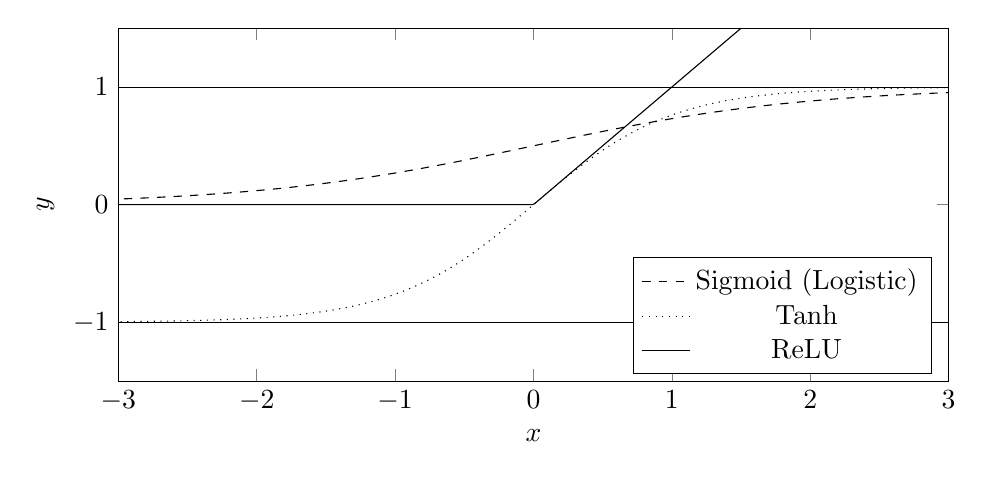
\begin{tikzpicture}
    \begin{axis}[xlabel=$x$,
    ylabel=$y$,
    width=\linewidth,
    height=0.5\linewidth,
    xmin=-3,
    xmax=3,
    ymin=-1.5,
    ymax=1.5,
	legend style={at={(0.98,0.02)},anchor=south east}    
    ]

	\addplot [samples=600, dashed] {1/(1+exp(-x))};
	\addlegendentry{Sigmoid (Logistic)}
	\addplot [samples=600, dotted] {(exp(x)-exp(-x))/(exp(x)+exp(-x))};
	\addlegendentry{Tanh}
    \addplot [samples=600] {max(x,0};
    \addlegendentry{ReLU}
    \addplot [samples=600, line width=0.01mm] {1};
    \addplot [samples=600, line width=0.01mm] {-1};
    \end{axis}
\end{tikzpicture}
\end{center}

\subsection{Artificial Neural Networks (ANNs)}

\mportant{$f(\vec{x};\vec{w},\theta):=\sum\limits_{j=1}^mw_j\underbrace{\phi(\theta_j^T\vec{x})}_{v_j}$}

\myspic{0.7}{Indexing}

\subsubsection{Forward Propagation}

\begin{enumerate}
\ncompaq
\item For each unit $j$ on input layer, set its value $v_j=x_j$
\item For each layer $l=1:L-1$
\begin{itemize}
\ncompaq
\item For each unit $j$ on layer $l$ set its value
\mportant{$v_j=\phi\left(\underbrace{\sum\limits_{i\in\text{Layer}_{l-1}}w_{j,i}v_i}_{z_j}\right)$}
\end{itemize}
\item For each unit $j$ on output layer, set its value
\mportant{$f_j=\sum\limits_{i\in\text{Layer}_{L-1}}w_{j,i}v_i$}
\item Predict
\begin{align*}
y_j&=f_j\text{ for regression}\\
y_j&=\sign{f_j}\text{ for classification}\\
y_j&=\text{argmax}(f_j)\text{ for multiclass classification}
\end{align*}
\end{enumerate}

In short:

\begin{enumerate}
\ncompaq
\item For input layer: $\vec{v}^{(0)}=\vec{x}$
\item For each hidden layer $l=1:L-1$
\begin{align*}
\vec{z}^{(l)}&=\vec{W}^{(l)}\vec{v}^{(l-1)}\\
\vec{v}^{(l)}&=\phi\left(\vec{z}^{(l)}\right)
\end{align*}
\item For output layer: $f=\vec{W}^{(l)}\vec{v}^{(L-1)}$
\item Predict: $\vec{y}=\vec{f}(\text{regression})$ or $\vec{y} = \sign{\vec{f}}$(class.) or $\vec{y}=\text{argmax} f_j$ (multiclass.)
\end{enumerate}

\subsubsection{Universal Approximation Theorem}

\begin{theorem}
Let $\sigma$ be any continuous sigmoidal function. Then finite sums of the form

\[G(x)=\sum\limits_{j=1}^N\alpha_j\sigma(y_j^Tx+\theta_j)\]

are dense in $C(I_n)$. In other words, given any $f\in C(I_n)$ and $\epsilon>0$, there is a sum, $G(x)$ of the above form for which

\[|G(x)-f(x)|<\epsilon\qquad\forall\quad x\in I_n\]

Thus the ANN can approximate any continuous function.
\end{theorem}

\subsection{How to train}

Given $D=\{(\vec{x}_1,y_1),\ldots,(\vec{x}_n,y_n)\}$ we want to optimize the weights: $\vec{W}=(\vec{W}^{(1)},\ldots,\vec{W}^{(L)})$.

\begin{itemize}
\ncompaq
\item Apply loss function
\mportant{$l(\vec{W};\vec{y},\vec{x})=l(\vec{y}-f(\vec{x},\vec{W}))$}
\item Optimize the weights to minimize loss over $D$

\mportant{$\vec{W}^\ast=\Argmin{\vec{W}}{\sum\limits_{i=1}^nl(\vec{W};\vec{y}_i,\vec{x}_i)}$}

for multiple outputs, define loss as sum of per-output losses.
\end{itemize}

\textbf{This problem is non-convex, thus there is no guarantee for finding the globally optimal solution.}

\subsubsection{Stochastic Gradient Descent}

\mportant{$\vec{W}^\ast=\Argmin{\vec{W}}{\sum\limits_{i=1}^nl(\vec{W};\vec{y}_i,\vec{x}_i)}$}

\begin{enumerate}
\ncompaq
\item Initialize weights $\vec{W}$
\item for $t=1,2,\ldots$
\begin{itemize}
\ncompaq
\item Pick data point $(\vec{x},\vec{y})\in D$ uniformly at random
\item Take step in negative gradient direction
\mportant{$\vec{W}\leftarrow\vec{W}-\eta_t\nabla_{\vec{W}}l(\vec{W};\vec{y},\vec{x})$}
\end{itemize}
\end{enumerate}

\paragraph{How to compute the gradient?}

Simple example featuring one input, one hidden and one output unit:

\mportant{$f(x,\vec{W})=w\overbrace{\phi(\underbrace{w'x}_z)}^v$}

\myspic{0.7}{Pictures/SimpleANN}

\begin{align*}
D&=\{(x,y)\}\\
L(w',w)&=l_y(f)=(f-y)^2\\
\frac{\partial L}{\partial w}&=\underbrace{\frac{\partial L}{\partial f}}_{\delta}\frac{\partial f}{\partial w}=\underbrace{l_y'(f)}_\delta v=\underbrace{2(f-y)}_\delta v\\
\frac{\partial L}{\partial w'}&=\underbrace{\frac{\partial L}{\partial f}}_{\delta}
\underbrace{\frac{\partial f}{\partial v}}_w
\frac{\partial v}{\partial w'}=\underbrace{\delta w\phi'(z)}_{\delta'} x
\end{align*}

Where the only two things not computed in forward propagation are the error signal from the output layer and the derivatives of the loss and the activation functions.

\textbf{More complicated example}

\mportant{$L=\sum\limits_{i}^2 l_i\left(\underbrace{\sum\limits_j^2 w_{i,j}\overbrace{\phi\left(\sum\limits_k^2 \underbrace{w_{j,k}'x_k}_{z_k}\right)}^{v_j}}_{f_i}\right)$}

\begin{align*}
\frac{\partial L}{\partial w_{i,j}}&=\underbrace{\frac{\partial L}{\partial f_i}}_{\delta_i}\frac{\partial f_i}{\partial w_{ij}}=\underbrace{l_i'(f_i)}_{\delta_i}v_j\\
\frac{\partial L}{\partial w_{jk}'}&=\sum\limits_i\underbrace{\frac{\partial L}{\partial f_i}}_{\delta_i}\frac{\partial f_i}{\partial v_j}\frac{\partial v_j}{\partial w_{jk}'}=\underbrace{\sum\limits_{i=1}^2\delta_i w_{i,j}\phi'(z_j)}_{\delta_j'}x_k
\end{align*}

\paragraph{Backpropagation}

\begin{enumerate}
\ncompaq
\item For each unit on the output layer
\begin{itemize}
\ncompaq
\item Compute error signal $\delta_j=l'_j(f_j)$
\item For each unit $i$ on layer $L$, $\frac{\partial L}{\partial w_{j,i}}=\delta_j v_i$
\end{itemize}
\item For each unit $j$ on hidden layer $l=L-1:-1:1$
\begin{itemize}
\ncompaq
\item Compute error signal $\delta_j=\phi'(z_j)\sum\limits_{i\in\text{Layer}_{l+1}}w_{i,j}\delta_i$
\item For each unit $i$ on layer $l-1$, $\frac{\partial L}{\partial w_{j,i}}=\delta_j v_i$
\end{itemize}
\end{enumerate}

This can be formulated in matrix form:

\begin{enumerate}
\ncompaq
\item For the output layer
\begin{itemize}
\ncompaq
\item Compute error: $\delta^{(L)}=\vec{l}'(\vec{f})=[l'(f_1),\ldots,l'(f_p)]$
\item Gradient $\nabla_{\vec{W}^{(L)}}l(\vec{W};\vec{y},\vec{x})=\delta^{(L)}\vec{v}^{(L-1)T}$
\end{itemize}
\item For each hidden layer $l=L-1:-1:1$
\begin{itemize}
\ncompaq
\item Compute error $\delta^{(l)}=\phi'\left(\vec{z}^{(l)}\right)\bigodot\left(\vec{W}^{(l+1)T}\delta^{(l+1)}\right)$

where $\bigodot$ is pointwise multiplication.
\item Gradient $\nabla_{\vec{W}^{(l)}}l(\vec{W};\vec{y},\vec{x})=\delta^{(l)}\vec{v}^{(l-1)T}$
\end{itemize}
\end{enumerate}

\subsection{Initializing Weights}

\begin{itemize}
\ncompaq
\item Non-convex problem, thus initialization matters
\item Random initialization usually works well
\begin{itemize}
\ncompaq
\item Glorot (tanh): \mportant{$w_{i,j}\sim\mathcal{N}(0,1/(n_{in}))$\\$w_{i,j}\sim\mathcal{N}(0,2/(n_{in}+n_{out}))$}
\item He (ReLU): \mportant{$w_{i,j}\sim\mathcal{N}(0,2/n_{in})$}
\end{itemize}
\end{itemize}

\subsection{Learning Rate}

\mportant{$\vec{W}\leftarrow\vec{W}-\eta_t\nabla_{\vec{W}}l(\vec{W};\vec{y};\vec{x})$}

\begin{itemize}
\ncompaq
\item Start with a fixed small learning rate and decrease slowly after some iterations.
\mportant{$\eta_t=\min(0.1,100/t)$}
\item Or a learning schedule, a piecewise constant learning rate, decreasing over time.
\end{itemize}

\subsubsection{Learning with Momentum}

\begin{itemize}
\ncompaq
\item Idea: Move not only into a direction of gradient, but also in direction of last weight update.
\mportant{$a\leftarrow m a+\eta_t\nabla_{\vec{W}}l(\vec{W};\vec{y};\vec{x})$\\$\vec{W}\leftarrow\vec{W}-\vec{a}$}

\begin{TDefinitionTable*}
$a$&Previous direction\\
$m$&Friction (\glqq forgetting\grqq previous $a$
\end{TDefinitionTable*}
\item This can help prevent oscillations.
\end{itemize}

\subsection{Weight-space Symmetries}

\begin{itemize}
\ncompaq
\item Multiple distinct weights compute the same predictions.
\item Therefore multiple local minima can be equivalent in terms of input-output mapping.
\end{itemize}

\subsection{Avoiding overfitting}

\begin{itemize}
\ncompaq
\item \textbf{Early stopping:} Don't run SGD until convergence.
\item \textbf{Regularization:} Add penalty term to keep weights small.
\item \textbf{Dropout:} Randomly ignore hidden units during each iteration of SGD with probability 1/2. After training half the weights to compensate.
\end{itemize}

\subsection{Batch normalization [Ioffe \& Szegedy 2015]}

\begin{itemize}
\ncompaq
\item Idea: normalize inputs to each layer according to mini-batch statistics.
\item Reduces internal covariate shift
\item Enables larger learning rates
\item Helps with regularization
\end{itemize}

\subsection{Convolutional Neural Networks}

The motivation for constructing CNNs is to use the invariant properties of convolution operations for ANNs such that they achieve a certain independency towards scaled or rotated features. The main idea is to implement a convolution layer by limiting interaction to nearby nodes.

\begin{define}
\textbf{Pooling} describes the process of reducing the number of parameters of a neural network by gathering subsets of nodes to form a single new node with a certain process (for example $\max()$).
\end{define}

\importname{Output dimension}{$\left(\frac{n+2p-f}{s},m\right)$}

where $p$ is the padding, $n$ is the number of pixels in $I\in\mathbb{R}^{n\times n}$, $s$ is the stride, $f$ describes the filter size of $F\in\mathbb{R}^{f\times f}$ and $m$ describes the number of filters applied.

\section{Clustering}

Idea: group data points into clusters such that similar points are in the same clusters and dissimilar points are in different clusters.

\begin{define}
The \textbf{hierachical} approach builds a clustering tree (bottom-up or top down) representing distances among data points.
\end{define}

\begin{define}
The \textbf{partitional} approach defines an optimizes a notion of \glqq cost\grqq defined over partitions. Basically you build a graph between points and then cut it (for example you make a cut to receive non-trivial partitions and try to minimize the number of edges cut).
\end{define}

\begin{define}
The \textbf{model based} approach maintains cluster \glqq models\grqq and infers cluster membership, for example assigning each point to the closest cluster-center.
\end{define}

\subsection{K-Means Clustering}

\begin{itemize}
\ncompaq
\item Represent each cluster by a single point.
\item Assign points to closest center
\item Assumes points are in Euclidean space $\vec{x}_i\in\mathbb{R}^d$
\item Represents clusters as centers $\mu_j\in\mathbb{R}^d$
\end{itemize}

\importabflex{c}{$\hat{R}(\mu)=\hat{R}(\mu_1,\ldots,\mu_k)=\sum\limits_{i=1}^n\min\limits_{j\in\{1,\ldots,k\}}||\vec{x}_i-\mu_j||_2^2$\\$\hat{\mu}=\text{arg}\min\limits_{\mu}\hat{R}(\mu)$}

\begin{itemize}
\ncompaq
\item $K$-Median clustering is particularly robust to outliers.
\end{itemize}

\subsubsection{Lloyd's Heuristic}

\begin{enumerate}
\ncompaq
\item Initialize cluster centers $\mu^{(0)}=[\mu^{(0)},\ldots,\mu_k^{(0)}]$
\item while not converged
\begin{itemize}
\ncompaq
\item Assign each point $\vec{x}_i$ to the closest center

\mportant{$z_i\leftarrow\text{arg}\min\limits_{j\in\{1,\ldots,k\}}||\vec{x}_i-\mu_j^{(t-1)}||_2^2$}
\item Update center as mean of assigned data points
\mportant{$\mu_j^{(t)}\leftarrow\frac{1}{n_j}\sum\limits_{i:z_i=j}\vec{x}_i$}
\end{itemize}
\end{enumerate}

\subsubsection{Properties}

\begin{itemize}
\ncompaq
\item Guaranteed to monotonically decrease average squared distance in each iteration.
\item Converges to a local optimum, which means it is sensitive to initialization.
\item Complexity per iteration $\mathcal{O}(nkd)$
\item The number of iterations required can be exponential.
\item Determining the number of clusters is hard.
\end{itemize}

\subsection{Adaptive Seeding (K-Means++)}

Random seeding can result in two problems: Clusters without centers and clusters with multiple centers. For that reason adaptive seeding is used:

\begin{enumerate}
\ncompaq
\item Start with a random data point as center.
\item Add centers $2$ to $k$ randomly, proportionally to the squared distance to closest selected center. Those points are sampled with the following probability, where $D(x)$ denotes the shortest distance from a data point to the closest center we have already chosen

\mportant{$P=\frac{D(x)^2}{\sum\limits_{x\in X}(x)^2}$}

Thus the probability to choose a new center far away from all others is more likely, and also clusters with many points are more likely to receive a closeby center.
\end{enumerate}

\paragraph{How to determine $k$ (Ellbow method)}

The heuristic for determining $k$ is based on the point at which the reduction in the $k$-means cost function begins to reduce slower. This is chosen as the optimal number of clusters. The same result can be achieved by adding a regularization term and find the minimum of that cost function.

\section{Dimensionality Reduction}

Given data set $D=\{\vec{x}_1,\ldots,\vec{x}_n\}$ obtain \glqq embedding\grqq (low dimensional representation $\vec{z}_1,\ldots,\vec{z}_n\in\mathbb{R}^k$.

\subsection{Approach}

\begin{itemize}
\ncompaq
\item Assume $D=\{\vec{x}_1,\dots,\vec{x}_n\}\subseteq\mathbb{R}^d$
\item Obtain mapping $\vec{f}:\mathbb{R}^d\rightarrow\mathbb{R}^k$ where $k\ll d$
\item Distinguish between
\begin{itemize}
\ncompaq
\item Linear dimension reduction: $\vec{f}(\vec{x})=\vec{A}\vec{x}$
\item Nonlinear dimension reduction (parametric or non-parametric.
\end{itemize}
\item The goal in dimension reduction is using a mapping that allows the reconstruction of the original data. The mapping should compress the data.
\begin{itemize}
\ncompaq
\item A simple example of a good compression is 2D data that can be fit with a line. A possible dimension reduction is to represent data points by their projection onto the fitted line.
\end{itemize}
\end{itemize}

\subsection{Linear dimensionality reduction}

\begin{itemize}
\ncompaq
\item $D=\{\vec{x}_1,\ldots,\vec{x}_n\}\subseteq\mathbb{R}^d$
\item Want $z_i\vec{w}\approx\vec{x}_i$ e.g. minimizing $||z_i\vec{w}-\vec{w}_i||_2^2$
\item To ensure uniqueness normalize $||\vec{w}||_2 = 1$
\item Optimize over $\vec{w},z_1,\ldots,z_n$ jointly:

\mportant{$(\vec{w}^\ast,\vec{z}^\ast)=\text{arg}\min\limits_{||\vec{w}||_2=1, z_1,\ldots, z_n\in\mathbb{R}}\sum\limits_{i=1}^n||\vec{x}_i-z_i\vec{w}||_2^2$}
\item Then, given a certain direction $\vec{w}$ the optimal $z$ can be found as

\mportant{$z_i^\ast=\vec{w}^T\vec{x}_i$}

Thus we effectively solve a regression problem, interpreting $x$ as features and $z$ as labels.

Inserting the above in the initial optimization results in

\mportant{$\vec{w}^\ast=\text{arg}\max\limits_{||\vec{w}||_2=1}\sum\limits_{i=1}^n(\vec{w}^T\vec{x}_i)^2$}

which can be further simplified to

\mportant{$\vec{w}^\ast=\text{arg}\max\limits_{||\vec{w}||_2=1}\vec{w}^T\Sigma\vec{w}$}

where $\Sigma=\frac{1}{n}\sum\limits_{i=1}^n\vec{x}_i\vec{x}_i^T$ is the \textbf{empirical covariance} assuming the data is centered: $\mu=\frac{1}{n}\sum\limits_i \vec{x}_i=0$.

\vspace{3ex}

The closed form solution to the above problem is then given by the principal eigenvector of $\Sigma$ i.e. $\vec{w}^\ast=\vec{v}_1$ where $\lambda_1$ is the largest eigenvalue.
\item This idea can be generalized to $k>1$, thus projections to more than one dimension:
\end{itemize}

\subsection{Principal Component Analysis (PCA)}

\begin{itemize}
\ncompaq
\item Linear Dimensionality Reduction for multiple orthogonal directions.
\item \textbf{The data needs to be centered!}

\important{$\mu=\frac{1}{n}\sum\limits_i x_i=0$}
\end{itemize}

\mportname{Empirical Covariance}{$\Sigma=\frac{1}{n} \sum\limits_{i=1}^{n}x_jx_i^T=\frac{1}{n}\begin{bmatrix}
x_1&\cdots&x_n
\end{bmatrix}\begin{bmatrix}
x_1^T\\\vdots\\x_n^T
\end{bmatrix}$}

\mportant{$(\vec{W},\vec{z}_1,\ldots,\vec{z}_n)=\text{arg}\min\sum\limits_{i=1}^n||\vec{W}\vec{z}_i-\vec{x}_i||_2^2$}

where $\vec{W}\in\mathbb{R}^{d\times k}$ is orthogonal, $\vec{z}_1,\ldots,\vec{z}_n\in\mathbb{R}^k$ and is given by $\vec{W}=(\vec{v}_1|\ldots|\vec{v}_k)$ and $\vec{z}_i=\vec{W}^T\vec{x}_i$ where 

\mportant{$\Sigma = \sum\limits_{i=1}^n\lambda_i\vec{v}_i\vec{v}_i^T\qquad\lambda_1\geq\ldots\geq\lambda_d\geq 0$}

This projection is chosen to minimize the reconstruction error (measured in Euclidean norm). The eigenvectors of the covariance matrix can be found using SVD.

\mportant{$X^TX=VS^TU^TUSV^T=V\underbrace{S^TS}_DV^T$}

where the solution, the new basis can be found as the first $k$ columns of $V$.

\vspace{3ex}

$k$ can be chosen by cross validation. For visualization we can choose $k$ by inspection.

\begin{itemize}
\ncompaq
\item Comparing K-Means to PCA, one can say that PCA has orthogonal basis vectors, where K-Means has arbitrary basis vectors.
\end{itemize}

\subsection{Nonlinear Dimension Reduction}

We can use kernels to reduce nonlinear problems to linear ones.

Thus we apply feature maps to PCA in the following way

\begin{itemize}
\ncompaq
\item We'd like to solve

\mportant{$\Argmax{||\vec{w}||_2=1}{\vec{w}^T\vec{X}^T\vec{X}\vec{w}}=\Argmax{||\vec{w}||_2=1}{\sum\limits_{j=1}^n\alpha_j\phi(\vec{x}_j)}$}

\item Applying features maps: $\vec{w}=\sum\limits_{j=1}^n\alpha_j\phi(\vec{x}_j)$ and thus $||\vec{w}|_2^2=\alpha^T\vec{K}\alpha$

\item This can be simplified to

\mportant{$\Argmax{\alpha^T\vec{K}\alpha = 1}{\alpha^t\vec{K}^T\vec{K}\alpha}$}

where $K$ is the kernel matrix $k(\vec{x}_j,\vec{x}_i)=\phi(\vec{x}_j)^T\phi(\vec{x}_i)$.

\item And the final problem formulates as:

\important{$\alpha^\ast=\Argmax{\alpha^T\vec{K}\alpha=1}{\alpha^T\vec{K}^T\vec{K}\alpha}$}

For which the closed form solution can be found as

\mportant{$\alpha^\ast =\frac{1}{\sqrt{\lambda_1}}\vec{v}_1$}

where $\lambda_1$ is the principal/largest eigenvalue and $\vec{v}_1$ the corresponding eigenvector.
\end{itemize}

\subsubsection{Kernel PCA (general $k$)}

\begin{itemize}
\ncompaq
\item For general $k\geq 1$, the Kernel Principal Components are given by $\alpha^{(1)},\ldots,\alpha^{(k)}\in\mathbb{R}^n$

\mportant{where $\alpha^{(i)}=\frac{1}{\sqrt{\lambda_i}}\vec{v}_i$}

\mportant{$\vec{K}=\sum\limits_{i=1}^n\lambda_i\vec{v}_i\vec{v}_i^T\qquad \lambda_1\geq\cdots\geq\lambda_d\geq 0$}

\item A new data point is then projected as $\vec{z}\in\mathbb{R}^k$

\mportant{$z_i=\sum\limits_{j=1}^n\alpha_j^{(i)}k(\vec{x},\vec{x}_j)$}
\end{itemize}

\subsection{Autoencoders}

Key idea: try to learn the identity function $\vec{x}\approx f(\vec{x};\theta)$

\mportant{$f(\vec{x};\theta)=f_2(f_1(\vec{x};\theta_1);\theta_2)$}

\begin{TDefinitionTable*}
$f_1:\mathbb{R}^d\rightarrow\mathbb{R}^k$&encoder\\
$f_2:\mathbb{R}^k\rightarrow\mathbb{R}^d$&decoder\\
\end{TDefinitionTable*}

\begin{itemize}
\ncompaq
\item Neural Networt Autoencoders are ANNs with one output unit for each of the $d$ input units, and $k<d$ hidden units.
\item The goal is to optimize the weights, such that the output agrees with the input. For example you can minimize the square loss for training:

\mportant{$\min\limits_{\vec{W}}\sum\limits_{i=1}^n||\vec{x}_i-f(\vec{x}_i;\vec{W})||_2^2$}
\item If you use linear activation functions and a single hidden layer you end up with PCA.
\end{itemize}

\section{Statistical Perspective}

\subsection{Minimizing Generalization Error}

\begin{itemize}
\ncompaq
\item Fundamental assumption: Our data set is generated i.i.d.
\mportant{$(\vec{x}_i,y_i)\sim P(\vec{X},Y)$}
\item Goal: Find hypothesis $h:\mathcal{X}\rightarrow\mathcal{Y}$ that minimizes the prediction error

\mportant{$R(h)=\int P(\vec{x},y)l(y;h(\vec{x}))d\vec{x}dy=\mathbb{E}_{\vec{x},y}\left[l(y;h(\vec{x}))\right]$}
\end{itemize}

\subsubsection{Example: LSQ}

\mportname{Risk}{$R(h)=\mathbb{E}_{\vec{x},y}\left[(y-h(\vec{x}))^2\right]$}

Which $h$ minimizes the risk? The hypothesis $h^\ast$ is given by the conditional mean:

\important{$h^\ast(\vec{x})=\mathbb{E}\left[Y|\vec{X}=\vec{x}\right]$}

Thus if we can estimate a predictor from the training data to estimate the conditional distribution

\mportant{$\hat{P}(Y|\vec{X})$}

based on which we can predict the label $y$ for point $\vec{x}$

\important{$\hat{y}=\hat{\mathbb{E}}\left[Y|\vec{X}=\vec{x}\right]=\int\hat{P}(y|\vec{X}=\vec{x})ydy$}

A common approach is \textbf{parametric estimation:}

\begin{itemize}
\ncompaq
\item Choose a particular parametric form $\hat{P}(Y|\vec{X},\theta)$
\item Find the Maximum (conditional) Likelihood Estimation

\mportant{$\theta^\ast=\Argmax{\theta}{\hat{P}(y_1,\ldots,y_n|\vec{x}_1,\ldots,\vec{x}_n,\theta)}$}
\end{itemize}

\subsubsection{MLE for Conditional Linear Gaussian}

\begin{itemize}
\ncompaq
\item The negative log likelihood is given by
\mportant{$L(\vec{w})=-\log P(y_i|\vec{x}_i,\vec{w})=\frac{n}{2}\log(2\pi\sigma^2)+\sum\limits_{i=1}^n\frac{(y_i-\vec{w}^T\vec{x}_i)^2}{2\sigma^2}$}
\item Under the conditional linear gaussian assumption (noise is gaussian and iid), maximizing the likelihood is equivalent to LSQ estimation.
\end{itemize}

\subsection{Bias Variance Tradeoff}

\mportant{$\hat{h}_D=\Argmin{h\in\mathcal{H}}{\sum\limits_{(\vec{x},y)\in D}(y-h(\vec{x}))^2}$}

\mportant{$\expeo{D}{\expeo{\vec{X},Y}{(Y-\hat{h}_D(\vec{X})^2}}=\text{Bias}^2+\text{Variance}+\text{Noise}$}

\renewcommand{\arraystretch}{1.3}
\importable{
$\text{Bias}^2$&$=\expeo{\vec{X}}{\expeo{D}{\hat{h}_D(\vec{X})}-h^\ast(\vec{X})}^2$\\
$\text{Variance}$&$=\expeo{\vec{X}}{\expeo{D}{\left(\hat{h}_D(\vec{X})-\expeo{D}{\hat{h}_D(\vec{X})}\right)^2}}$\\
$\text{Noise}$&$=\expeo{\vec{X},Y}{Y-h^\ast(\vec{X})^2}$
}

\renewcommand{\arraystretch}{1}

\subsection{Bayesian Modelling}

\importname{Bayes' Rule}{$p(\vec{w}|\vec{x}_{1:n},y_{1:n})=\frac{p(\vec{w})p(y_{1:n}|x_{1:n},\vec{w})}{p(y_{1:n}|x_{1:n})}$}

where we assume that $\vec{w}$ is independent of $x$, thus $p(\vec{w})=p(\vec{w}|\vec{x}_{1:n})$. Note that the Bayes' rule in this case does not take $\vec{x}$ into account, but just deals with $y$ and $\vec{w}$.

Finding the parameters, that are most likely, given $\vec{x}_{1:n}, y_{1:n}$ and some a priori distribution of $\vec{w}$, is done my finding the argmax of $p(\vec{w}|\vec{x}_{1:n},y_{1:n})$.

\importabflex{l}{$\Argmax{\vec{w}}{p(\vec{w}|\vec{x}_{1:n},y_{1:n}})$\\$=\Argmin{\vec{w}}{\lambda||\vec{w}||_2^2+\sum\limits_{i=1}^n(y_i-\vec{w}^T\vec{x}_i)^2}$ for $\lambda=\frac{\sigma'^2}{\beta^2}$}

\begin{itemize}
\ncompaq
\item Ridge regression can be understood as finding the MAP parameter estimate for a linear regression problem, assuming that the noise $P(y|\vec{x},\vec{W})$ is i.i.d. Gaussian and the prior $P(\vec{w})$ on the model parameters $\vec{w}$ is Gaussian.
\end{itemize}

\mportant{$\Argmin{\vec{w}}{\sum\limits_{i=1}^n(y_i-\vec{w}^T\vec{w}_i)^2+\lambda||\vec{w}||_2^2}\equiv\Argmax{\vec{w}}{P(\vec{w}\prod\limits_iP(y_i|\vec{x}_i,\vec{w})}$}

\subsubsection{Regularization vs. MAP inference}

A regularized estimation can often be understood as MAP inference.

\begin{align*}
\Argmin{\vec{w}}{\sum\limits_{i=1}^nl(\vec{w}^T\vec{x}_i;\vec{x}_i,y_i)+C(\vec{w})}&=\Argmax{\vec{w}}{\prod\limits_{i}P(y_i|\vec{x}_i,\vec{w})P(\vec{w})}\\
&=\Argmax{\vec{w}}{P(\vec{w}|D)}\ (\text{Bayes})
\end{align*}

where $C(\vec{w})=-\log P(\vec{w})$ and $l(\vec{w}^T\vec{x}_i;\vec{x}_i,y_i)=-\log P(y_i|\vec{x}_i,\vec{w})$

\begin{center}
\begin{tabular}{ll}
Regularization&Prior\\
$l1$&Laplace
\end{tabular}
\end{center}

\subsection{Bayes' optimal classifier}

\begin{itemize}
\ncompaq
\item Assume the data is generated i.i.d. according to

\mportant{$(\vec{x}_i,y_i)\sim P(\vec{X},Y)$}
\item The hypthosis $h^\ast$ minimizing $R(h)=\mathbb{E}_{\vec{X},Y}\left[\left[Y\neq h(\vec{X})\right]\right]$ is given by the most probable class

\mportant{$h^\ast(x)=\Argmax{y}{P(Y=y|\vec{X}=\vec{x})}$}
\end{itemize}

\subsection{Logistic Regression}

\begin{itemize}
\ncompaq
\item Assumption: Bernoulli noise
\item Idea: Describe the probability of label $y$ using the linear model for classification and combining it with a link function that turns $\vec{w}^T\vec{x}$ into a probability:

\mportant{$P(y=+1|\vec{x})=\sigma(\vec{w}^T\vec{x})=\frac{1}{1+\exp (-\vec{w}^T\vec{x})}$}
\end{itemize}

\subsubsection{MLE for Logistic Regression}

\mportant{$\hat{\vec{w}}=\Argmax{\vec{w}}{\prod\limits_{i=1}^n P(y_i|\vec{x}_i,\vec{w})}$}

Idea: Choose $\vec{w}$ such that for all observations the certainty (probability of getting the correct label $y_i$ given feature vector $\vec{x}_i$) is as high as possible and optimize over all observations.

\vspace{3ex}

The negative log likelihood function can then be found as 

\mportant{$\hat{R}(\vec{w})=\sum\limits_{i=1}^n\log\left(1+\exp(-y_i\vec{w}^T\vec{x})\right)$}

Since this loss function is convex we can use optimization techniques like SGD.

\subsubsection{SGD for \textcolor{blue}{L2-Regularized} Logistic Regression}

\begin{enumerate}
\ncompaq
\item Intialize $\vec{w}$
\item For $t=1,2,\ldots$
\begin{enumerate}
\ncompaq
\item Pick data point $(\vec{x},y)$ uniformly at random from data $D$
\item Compute probability of misclassification with current model

\mportant{$\hat{P}(Y=-y|\vec{w},\vec{x})=\frac{1}{1+\exp(y\vec{w}^T\vec{x})}$}

\item Take gradient step

\mportant{$\vec{w}\leftarrow\vec{w}\textcolor{blue}{(1-2\lambda \eta_t)}+\eta_t y\vec{X}\hat{P}(Y=-y|\vec{w},\vec{x})$}
\end{enumerate}
\end{enumerate}

Now since we'd like to use a regularizer to control the model complexity we estimate MAP instead of MLE:

\begin{center}
\begin{tabular}{ll}
Prior&Regularizer\\
Gaussian&L2\\
Laplace&L1
\end{tabular}
\end{center}

\subsubsection{Kernelized Logistic Regression}

\begin{itemize}
\ncompaq
\item \textbf{Learning:} Find optimal weights by minimizing logistic loss and regularizer.

\mportant{$\hat{\alpha}=\Argmin{\alpha}{\sum\limits_{i=1}^n\log\left(1+\exp\left(-y_i\alpha^T\vec{K}_i\right)\right)+\lambda\alpha^T \vec{K}\alpha}$}
\item \textbf{Classification:} Use conditional distribution

\mportant{$\hat{P}(y|\vec{x},\alpha)=\frac{1}{1+\exp\left(-y\sum\limits_{j=1}^n \alpha_jk(\vec{x}_j,\vec{x})\right)}$}
\end{itemize}

\subsection{Multi-Class Logistic Regression}

\begin{itemize}
\ncompaq
\item Maintain one weight vector per class an model

\mportant{$P(Y=)i|\vec{x},\vec{w}_1,\ldots,\vec{w}_c)=\frac{\exp(\vec{w}_i^T\vec{x})}{\sum\limits_{j=1}^c\exp(\vec{w}_j^T\vec{x})}$}
\item Not unique - can enforce uniqueness by setting $\vec{w}_c=0$ (this recovers logistic regression as special case)
\item Corrsponding loss function (cross-entropy loss):

\mportant{$l(y;\vec{x},\vec{w}_1,\ldots,\vec{w}_c)=-\log P(Y=y|\vec{x},\vec{w}_1,\ldots,\vec{w}_c)$}
\end{itemize}

\subsection{SVM vs. Logistic Regression}

\begin{itemize}
\ncompaq
\item SVM / Perceptron
\begin{itemize}
\ncompaq
\item[+] Sometimes higher classification accuracy
\item[+] Sparse solutions
\item[-] Can't (easily) get class probabilites
\end{itemize}
\item Logistic Regression
\begin{itemize}
\ncompaq
\item[+] Can obtain class probabilities
\item[-] Dense solutions
\end{itemize}
\end{itemize}

\subsection{Different Loss Functions}

\begin{center}
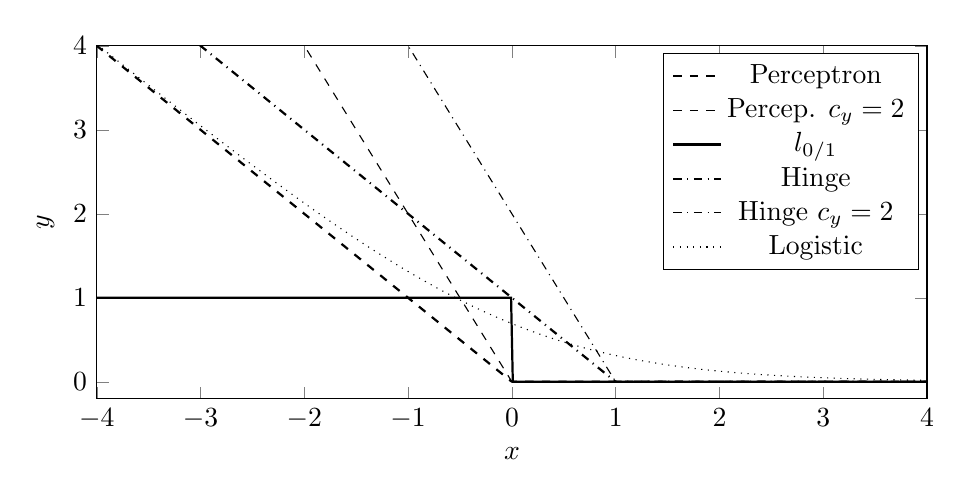
\begin{tikzpicture}
    \begin{axis}[xlabel=$x$,
    ylabel=$y$,
    width=\linewidth,
    height=0.5\linewidth,
    xmin=-4,
    xmax=4,
    ymin=-0.2,
    ymax=4,
	legend style={at={(0.99,0.98)},anchor=north east},
	ylabel near ticks, 
	ylabel shift={0pt},
	declare function={
    l(\x)= (\x < 0) * (1) + (\x >= 0) * (0);
  }   
    ]

	\addplot [samples=600, dashed, thick] {max(0,-x)};
	\addlegendentry{Perceptron}
	\addplot [samples=600, dashed] {2*max(0,-x)};
	\addlegendentry{Percep. $c_y=2$}
	\addplot [samples=600, thick] {l(x)};
	\addlegendentry{$l_{0/1}$}
    \addplot [samples=600, dash dot, thick] {max(0,1-x)};
    \addlegendentry{Hinge}
    \addplot [samples=600, dash dot] {2*max(0,1-x)};
    \addlegendentry{Hinge $c_y=2$}
    \addplot [samples=600, dotted] {ln(1+exp(-x))};
    \addlegendentry{Logistic}
    \end{axis}
\end{tikzpicture}
\end{center}

\section{Bayesian Decision Theory}

\begin{itemize}
\ncompaq
\item Given:
\begin{itemize}
\ncompaq
\item Conditional distribution over labels $P(y|\vec{x})$
\item Set of actions $\mathcal{A}$
\item Cost function $C:\mathcal{Y}\times\mathcal{A}\rightarrow\mathbb{R}$
\end{itemize}
\item Bayesian Decision Theory recommends to pick the action that minimizes the expected cost

\mportant{$a^\ast=\Argmin{a\in\mathcal{A}}{\mathbb{E}_y\left[C(y,a)|\vec{x}\right]}$}
\item If we had access to the true distribution $P(y|\vec{x})$ this decision implements the \textbf{Bayesian Optimal Decision}.
\end{itemize}

\subsection{Example with Logistic Regression}

\begin{itemize}
\ncompaq
\item Est. cond. dist: $\hat{P}(y|\vec{x})=\text{Ber}(y;\sigma(\hat{\vec{w}}^T\vec{x}))$
\item Action set: $\mathcal{A}=\{+1,-1\}$
\item Then the action that minimizes the expected cost is the most likely class:

\mportant{$a^\ast=\Argmax{y}{\hat{P}(y|\vec{x})=\text{sign}(\vec{w}^T\vec{x})}$}
\end{itemize}

\subsection{Asymmetric Cost}

\mportant{$C(y,a)=\begin{cases}
c_{FP}&\text{ if }y=-1\text{ and }a=+1\\
c_{FN}&\text{ if }y=+1\text{ and }a=-1\\
0&\text{ otherwise}\end{cases}$}

which is equivalent to

\mportant{$C(y,a)=c_{FN}\max(y-a,0)+c_{FP}\max(a-y,0)$}

Then the action that minimizes the cost is

\begin{align*}
c_+&=\mathbb{E}_Y\left[c(Y,+1)|\vec{x}\right]=c_{FP}P(Y=-1|\vec{x})=c_{FP}(1-p)\\
c_-&=\mathbb{E}_Y\left[c(Y,-1)|\vec{x}\right]=c_{FN}P(Y=+1|\vec{x})=c_{FN} p
\end{align*}

Therefore we predict $+1$ if $c_+<c_-$ and vice versa.

\begin{align*}
c_+&<c_-\\
c_{FP}(1-p)&<c_{FN}p\\
p&>\frac{c_{FP}}{c_{FP}+c_{FN}}
\end{align*}

\subsubsection{Doubtful Logistic Regression}

\textbf{Idea:} Pick most likely class only if confident enough.

\begin{itemize}
\ncompaq
\item Est. cond. dist.: $\hat{P}(y|\vec{x})=\text{Ber}(y;\sigma(\hat{\vec{w}}^T\vec{x}))$
\item Action set: $\mathcal{A}=\{+1,-1,D\}$
\item Cost functions:

\mportant{$C(y,a)=\begin{cases}
[y\neq a]&\text{ if }a\in\{+1,-1\}\\
c&\text{ if }a=D
\end{cases}$}
\item the the action that minimizes the expected cost is given by

\mportant{$a^\ast=\begin{cases}
y&\text{ if }\hat{P}(y|\vec{x})\geq 1-c\\
D&\text{ otherwise}
\end{cases}$}
\end{itemize}

\section{Generative vs. Discriminative Modelling}

\textbf{Idea:} Model $P(\vec{x})$ to gain the capability of detecting outliers (unusual points for which $P(\vec{x})$ is very small), since models only estimating conditional distributions $P(y|\vec{x})$ can't do that.

\begin{define}
\textbf{Discriminative models} aim to estimate $P(y|\vec{x})$.
\end{define}

\begin{define}
\textbf{Generative models} aim to estimate the joint distribution $P(y,\vec{x})$.
\end{define}

\subsection{Typical Approach on Generative Modelling}

\begin{enumerate}
\ncompaq
\item Estimate prior on labels $P(y)$.
\item Estimate conditional distribution $P(\vec{x}|y)$ for each class.
\item Obtain predictive distribution using Bayes' rule:

\mportant{$P(y|\vec{x})=\frac{1}{Z = P(x)}P(y)P(\vec{x}|y)$}
\end{enumerate}

\textbf{We can derive the conditional distribution from the joint distribution but not vice versa!}

\subsection{Gaussian Naive Bayes Model $p(\vec{x}_i,y)=p(\vec{x}_i|y)p(y)$}

\begin{itemize}
\ncompaq
\item \textbf{Used for continuous features!} If not use categorical model.
\item Model class label as generated from categorical variable

\mportant{$P(Y=y)=p_y\qquad q\in\mathcal{Y}=\{1,\ldots,c\}$}

Assumption: Features are conditionally independent if the class label is known. ($\Sigma_y=\text{diag}(\cdots)$)

\item \textbf{Learning:} Given data $D=\{(\vec{x}_1,y_1),\ldots,(\vec{x}_n,y_n)\}$
\begin{itemize}
\ncompaq
\item MLE for class prior: 

\mportant{$\hat{P}(Y=y)=\hat{p}_y=\frac{\text{Count}(Y=y)}{n}$}
\item MLE for feature distribution:
\begin{align*}
\hat{P}(x_i|y)&=\mathcal{N}(x_i;\hat{\mu}_{y,i},\sigma_{y,i}^2)\\
\hat{\mu}_{y,i}&=\frac{1}{\text{Count}(Y=y)}\sum\limits_{j:y_i=y}x_{j,i}\\
\sigma_{y,i}^2&=\frac{1}{\text{Count}(Y=y)}\sum\limits_{j:y_j=y}(x_{i,j}-\hat{\mu}_{y,i})^2
\end{align*}

where $x_{j,i}$ represents the value of feature $i$ for instance $j\ (x_j,y_i)$.
\end{itemize}
\item \textbf{Prediction} given point $\vec{x}$

\mportant{$y=\Argmax{y'}{\hat{P}(y'|\vec{x})}=\Argmax{y'}{\hat{P}(y')\prod\limits_{i=1}^n\hat{P}(x_i|y')}$}
\item Decision Rules for binary classification

\mportant{$y=\text{sign}\left(\log\frac{P(Y=1|\vec{x})}{P(Y=-1|\vec{x})}\right)$}

It is easy to verify that the above returns $+1$ if $P(Y=1|\vec{x})>=0.5$.

\begin{define}
The function $f(\vec{x})=\log\frac{P(Y=1|\vec{x})}{P(Y=-1|\vec{x})}$ is called \textbf{discriminant function}.
\end{define}
\item GNB ($c=2$), in case of shared variance, produces a linear classifier:

\mportant{$f(\vec{x})=\vec{w}^T\vec{x}+w_0$}

where $w_0=\log\frac{\hat{p}_+}{1-\hat{p}_+}+\sum\limits_{i=1}^d\frac{\hat{\mu}_{-,i}^2-\hat{\mu}_{+,i^2}}{2\hat{\sigma}_i^2}$ and $w_i=\frac{\mu_{+,i}-\mu_{-,i}}{\sigma_i^2}$
\item Connection of discriminant function, class probability and link function:

\mportant{$P(Y=1|\vec{x})=\frac{1}{1+\exp(-f(\vec{x}))}=\sigma(f(\vec{x}))$}
\item GNB with shared variance and $c=2$ will make the same predictions as logistic regression if the model assumptions are met.
\end{itemize}

\subsubsection{Issue with NBM}

\begin{itemize}
\ncompaq
\item If there is a conditional correlation between class labels, then the assumption of independence between features is violated.
\item Due to the independence assumption predictions can become overconfident.
\item This is alright if we care only about the most likely class, but not if we want to use probabilities for making decisions (e.g. asymmetric losses etc).
\end{itemize}

\subsection{Gaussian Bayes Classifiers (not naive)}

\begin{itemize}
\ncompaq
\item In contrast to GNB general gaussian bayes classifiers model features as generated by multivariate Gaussians

\mportant{$P(\vec{x}|y)=\mathcal{N}(\vec{x};\mu_y,\Sigma_y)$}
\item \textbf{Learning} given $D=\{(\vec{x}_1,y_1),\ldots,(\vec{x}_n,y_n)\}$
\begin{itemize}
\ncompaq
\item MLE for class label distribution

\mportant{$\hat{P}(Y=y)=\hat{p}_y=\frac{\text{Count}(Y=y)}{n}$}
\item MLE for feature distribution

\begin{align*}
\hat{P}(\vec{x}|y)&=\mathcal{N}(\vec{x};\hat{\mu}_y,\hat{\Sigma}_y)\\
\hat{\mu}_y&=\frac{1}{\text{Count}(Y=y)}\sum\limits_{i:y_i=y}\vec{x}_i\\
\hat{\Sigma}_y&=\frac{1}{\text{Count}(Y=y)}\sum\limits_{i:y_i=y}(\vec{x}_i-\hat{\mu}_y)(\vec{x}_i-\hat{\mu}_y)^T
\end{align*}
\end{itemize}
\item Discriminant functions for GBCs
\begin{itemize}
\ncompaq
\item Want: $f(\vec{x})=\log\frac{P(Y=1|\vec{x})}{P(Y=-1|\vec{x})}$
\item This is given by

\mportant{\tiny$f(\vec{x})=\log\frac{p}{1-p}+\frac{1}{2}\left[\log\frac{|\hat{\Sigma}_-|}{|\hat{\Sigma}_+|}+\left((\vec{x}-\hat{\mu}_-)^T\hat{\Sigma}_-^{-1}(\vec{x}-\hat{\mu})\right)-\left((\vec{x}-\hat{\mu}_+)^T\hat{\Sigma}_+^{-1}(\vec{x}-\hat{\mu}_+)\right)\right]$\normalsize}

where $p=P(Y=1)$.
\end{itemize}

\end{itemize}

\subsection{Fisher's Linear Discriminant Analysis}

Assumptions:

\begin{itemize}
\ncompaq
\item $p=0.5, c = 2$
\item Equal covariances $\hat{\Sigma}_-=\hat{\Sigma}_+=\hat{\Sigma}$
\end{itemize}

\mportant{$f(\vec{x})=\vec{x}^T\underbrace{\hat{\Sigma}^{-1}(\hat{\mu}_+-\hat{\mu}_-)}_{\vec{w}}+\underbrace{\frac{1}{2}(\hat{\mu}_-^T\hat{\Sigma}^{-1}\hat{\mu}_--\hat{\mu}_+^T\hat{\Sigma}^{-1}\hat{\mu}_+)}_{w_0}$}

Under these circumstances the prediction is

\mportant{$y=\text{sign}(f(\vec{x}))=\text{sign}(\vec{w}^T\vec{x}+w_0)$}

\begin{itemize}
\ncompaq
\item If the model assumptions are met, LDA will make the same predictions as Logistic Regression.
\item \textbf{LDA vs. PCA}: LDA can be viewed as a projection to a 1-dimensional subspace that maximizes the ratio of between-class an within-class variances (very little variance within classes, alot across classes), where in contrast PCA $(k=1)$ maximizes the variance of the resulting 1-dimensional projection. PCA does not separate the classes.
\end{itemize}

\subsection{Quadratic Discriminant Analysis}

In the general case 

\mportant{$f(\vec{x})=\log\left(\frac{p}{1-p}\right)+\frac{1}{2}\left[\log\left(\frac{|\hat{\Sigma}_-|}{|\hat{\Sigma}_+|}\right)+\left((\vec{x}-\hat{\mu}_-)^T\hat{\Sigma}_-^{-1}(\vec{x}-\hat{\mu}_-)\right)-\left((\vec{x}-\hat{\mu}_+)^T\hat{\Sigma}_+^{-1}(\vec{x}-\hat{\mu}_1)\right)\right]$}

and we predict

\mportant{$y=\text{sign}(f(\vec{x}))$}

which is called \textbf{quadratic discriminant analysis.}

\subsection{General Comparison}

\begin{itemize}
\ncompaq
\item Fisher's LDA
\begin{itemize}
\ncompaq
\item Generative models, i.e. models $P(\vec{X},Y)$
\item[+] Can be used to detect outliers: $P(\vec{X})<t$
\item[$\bullet$] Assumes normality of $\vec{X}$
\item[-] Not very robust against violation of this assumption
\end{itemize}
\item Logistic Regression
\begin{itemize}
\ncompaq
\item[$\bullet$] Discriminative model, i.e. models $P(Y|\vec{X})$ only
\item[-] Cannot detect outliers
\item[$\bullet$] Makes no assumptions on $\vec{X}$
\item[+] More robust
\end{itemize}
\item Gaussian Naive Bayes Models
\begin{itemize}
\ncompaq
\item[-] Conditional independence assumption may lead to overconfidence 
\item[+] Predictions might still be useful
\item[+] Number of parameters = $O(c d)$
\item[$\bullet$] Complexity (memory + interface) is linear in $d$
\end{itemize}
\item General Gaussian Bayes Models
\begin{itemize}
\ncompaq
\item[+] Captures correlations among features
\item[+] Avoids overconfidence
\item[-] Number of parameters = $O(c d^2)$
\item[-] Complexity quadratic in $d$
\end{itemize}
\end{itemize}

\subsection{Adaptation to Discrete Features}

\begin{itemize}
\ncompaq
\item Suppose $X_i$ take discrete values
\item Since generative models allow to swap the distribution easily we can use different models like
\begin{itemize}
\ncompaq
\item Bernoulli
\item Categorical
\item Multinominal
\end{itemize}
\end{itemize}

\subsubsection{Categorical Naive Bayes Classifier}

\begin{itemize}
\ncompaq
\item  Model class labels as generated from categorical variable.

\mportant{$P(Y=y)=p_y\qquad y\in\mathcal{Y}=\{1,\ldots,c\}$}
\item Model features by (conditionally) independent categorical random variables

\mportant{$P(X_i=c|Y=y)=\theta_{c|y}^{(i)}$}

\item MLE for CNBC
\begin{itemize}
\ncompaq
\item Given $D\{(\vec{x}_1,y_1),\ldots(\vec{x}_n,y_n)\}$
\item MLE for class label distribution $\hat{P}(Y=y)=\hat{p}_y$

\mportant{$\hat{p}_y=\frac{\text{Count}(Y=y)}{n}$}
\item MLE for distribution of feature $i$ $\hat{P}(X_i=c|y)=\theta_{c|y}^{(i)}$

\mportant{$\theta_{c|y}^{(i)}=\frac{\text{Count}(X_i=c,Y=y)}{\text{Count}(Y=y)}$}

\item Prediction given new point $\vec{x}$

\mportant{$y=\Argmax{y'}{\hat{P}(y'|\vec{x})}=\Argmax{y'}{\hat{P}(y')\prod\limits_{i=1}^d\hat{P}(x_i|y')}$}
\end{itemize}
\end{itemize}

\subsubsection{Combination of Discrete and Continuous Features}

\begin{itemize}
\ncompaq
\item The (N)BC does not require each feature to follow the same type of conditional distribution
\item Training and prediction is the same as before
\end{itemize}

\subsection{Avoiding Overfitting of MLE}

\begin{itemize}
\ncompaq
\item Restrict Model Class (assumptions on covariance structure, e.g. GNB) thus using fewer parameters
\item Regularization is equivalent to putting a prior on the weights to describe class probabilities.
\end{itemize}

\subsubsection{Prior over parameters ($c=2$)}

\begin{itemize}
\ncompaq
\item Prior on class probabilities: $P(Y=1)=\theta$
\item MLE: $\hat{\theta}=\frac{\text{Count}(Y=1)}{n}$
\item Extreme case: $n=1$, in which case the empirical frequencies are not informative and the MLE collapses.
\item Solution: Assume prior knowledge in the form of a probability distribution $\rightarrow$ use beta priors.
\end{itemize}

\paragraph{Conjugate Distributions}

\begin{define}
A pair of prior distributions and likelihood functions is called \textbf{conjugate} if the posterior distribution remains in the same family as the prior.

\underline{This enables a simple and efficient calculation of prior distributions.}
\end{define}

\paragraph{Example}

\begin{itemize}
\ncompaq
\item Prior: Beta($\theta;\alpha_+,\alpha_-)$
\item Observations: Suppose we observe $n_+$ positive and $n_-$ negative labels.
\item Posterior: Beta($\theta;\alpha_++n_+,\alpha_-+n_-)$
\item thus $\alpha_+,\alpha_-$ act as pseudo-counts.
\end{itemize}

\paragraph{MAP estimate}

\mportant{$\hat{\theta}=\Argmax{\theta}{P(\theta|y_1,\ldots,y_n;\alpha_+,\alpha_-)}=\frac{\alpha_++n_+-1}{\alpha_++n_++\alpha_-+n_--2}$}

\paragraph{Conjugate Priors}

\begin{center}
\begin{tabular}{ll}
\textbf{Prior/Posterior}&\textbf{Likelihood function}\\
Beta&Bernoulli/Binomial\\
Dirichlet&Categorical/Multinomial\\
Gaussian (fixed covariance)&Gaussian\\
Gaussian-inverse Wishart&Gaussian\\
Gaussian process&Gaussian
\end{tabular}
\end{center}

\section{Dealing with Missing Data}

\subsection{Gaussian Mixtures}

\mportant{$P(\vec{x}|\theta)=P(\vec{x}|\mu,\Sigma,\vec{w})=\sum\limits_{i=1}^k w_i\mathcal{N}(\vec{x};\mu_i,\Sigma_i)$}

where $w_i\geq 0$ and $\sum\limits_iw_i=1$ and $P(\vec{x}|\theta)$ is a convex combination of gaussian distributions.

\mportname{MLE}{$(\mu^\ast,\Sigma^\ast,w^\ast)=\Argmin{}{-\sum\limits_{i}\log\sum\limits_{j=1}^k w_j\mathcal{N}(\vec{x}_i|\mu_j,\Sigma_j)}$}

\begin{itemize}
\ncompaq
\item This objective function is nonconvex.
\item Challenges for stochastic descent:
\begin{itemize}
\ncompaq
\item Convariance matrices must remain symmetric positive definite, which as constraints might be difficult to maintain
\end{itemize}
\item The joint distribution $P(z,\vec{x})=w_z\mathcal{N}(\vec{x}|\mu_z,\Sigma_z)$ is identical to the generative model used by the GBC.
\item If we have the labels to our training data, we can find the parameters by computing the MLE in closed form as done for GBC.
\item \textbf{Initialization:}
\begin{itemize}
\ncompaq
\item For weights: Uniform Distribution
\item For means: Random initialization or k-means++
\item For variances: Initialize as spherical, e.g. according to empirical variance in the data.
\end{itemize}
\item \textbf{Selecting $k$}: Similar challenge to selecting number of clusters, in contrast to k-means, here cross-validation works well. Aim to maximize log-likelihood on validation set.
\item \textbf{Degeneracy}: Given a single data point the loss converges to $-\infty$ as $\mu=x,\ \sigma\rightarrow 0$. Thus the optimal GMM chooses $k=n$ and puts one Gaussian around each data point with variance tending to 0. The solution lies in adding a small term to the diagonal of the MLE:

\mportant{$\Sigma_j^{(t)}\leftarrow \frac{\sum\limits_{i=1}^n\gamma_j^{(t)}(\vec{x}_i)(\vec{x}_i-\mu_j^{(t)})(\vec{x}_i-\mu_j^{(t)})^T}{\sum\limits_{i=1}^n \gamma_j^{(t)}(\vec{x}_i)}+\nu^2\mathbb{I}$}
\end{itemize}

\subsubsection{Hard-EM}

\begin{enumerate}
\ncompaq
\item Initialize the parameters $\theta^{(0)}$

where $\theta^{(\ast)}=\left[w_{1:c}^{(\ast)},\mu_{1:c}^{(\ast)},\Sigma_{1:c}^{(\ast)}\right]$.
\item For $t=1,2,\ldots$
\begin{enumerate}
\ncompaq
\item E-Step: Predict most likely class for each data point

\begin{align*}
z_i^{(t)}&=\Argmax{z}{P(z|\vec{x}_i,\theta^{(t-1)})}\\
&=\Argmax{z}{\underbrace{P(z|\theta^{(t-1)})}_{w_z^{(t-1)}}\underbrace{P(\vec{x}_i|z,\theta^{(t-1)})}_{\mathcal{N}(\vec{x}_i|\mu_z^{(t-1)},\Sigma_z^{(t-1)}}}
\end{align*}
\item Now we got complete data $D^{(t)}=\{(\vec{x}_1,z_1^{(t)}),\ldots,(\vec{x}_n,z_n^{(t)})\}$
\item M-Step: Compute MLE as for the GBC

\mportant{$\theta^{(t)}=\Argmax{\theta}{P(D^{(t)}|\theta)}$}
\end{enumerate}
\end{enumerate}

\paragraph{Problems with Hard EM}

\begin{itemize}
\ncompaq
\item[-] Points are assigned a fixed label, even though the model is uncertain.
\item[-] Intuitively, this tries to extract too much information from a single point.
\item In practice, this may work poorly if clusters are overlapping.
\end{itemize}

\paragraph{k-Means Algorithm vs. EM for GMM}

\begin{itemize}
\ncompaq
\item Can understand k-Means Algorithm (Lloyd's heuristic) as special case of Hard-EM for GMMs
\begin{itemize}
\ncompaq
\item Uniform weights over mixture components
\item Assuming identical, spherical covariance matrices
\end{itemize}
\item Can also understand k-Means Algorithm as limiting case of Soft-EM for GMM
\begin{itemize}
\ncompaq
\item Assumptions same as above, with additionally variances tending to 0
\end{itemize}
\end{itemize}

\[\gamma_j(\vec{x})=\begin{cases}1&\text{if $\mu_j$ i closest to $x$}\\0&\text{else}\end{cases}\]

\subsubsection{Posterior Probabilities}

\begin{itemize}
\ncompaq
\item Suppose we knew $P(z|\theta)$, the distribution of the labels given the model parameters and $P(\vec{x}|z,\theta)$, the distribution of the features given the labels and parameters.
\item Compute a posterior distribution over cluster membership, thus inferring distributions over latent (hidden) variables $z$.
\end{itemize}

\begin{align*}
\gamma_j(\vec{x})&=P(z|\vec{x},\Sigma,\mu,\vec{w})\\
&=\frac{p(\vec{x}|z,\theta)p(z|\theta)}{p(\vec{x}|\theta)}=\frac{w_jP(\vec{x}|\Sigma_j,\mu_j)}{\Sigma_lw_lP(\vec{x}|\Sigma_l,\mu_l}
\end{align*}

\begin{itemize}
\ncompaq
\item Hard EM takes the argmax of the above distribution, where Soft EM records the likelihood of each class for each point.
\end{itemize}

\subsection{Expectation-Maximization (Soft-EM)}

\begin{itemize}
\ncompaq
\item While not converged
\begin{enumerate}
\ncompaq
\item E-Step: Calculate cluster membership weights (\glqq Expected sufficient statistics\grqq  for each point (aka \glqq responsibilities\grqq))

Calculate $\gamma_j^{(t)}(\vec{x}_i)$ for each $i$ and $j$ given estimates of $\mu^{(t-1)},\Sigma^{(t-1)},\vec{w}^{(t-1)}$ from previous iteration
\item M-Step: Fit clusters to weighted data points (closed form Maximum likelihood solution)

\begin{align*}
w_j^{(t)}&\leftarrow \frac{1}{n}\sum\limits_{i=1}^n \gamma_j^{(t)}(\vec{x}_i)\\
\mu_j^{(t)}&\leftarrow \frac{\sum\limits_{i=1}^n\gamma_j^{(t)}(\vec{x}_i)\vec{x}_i}{\sum\limits_{i=1}^n\gamma_j^{(t)}(\vec{x}_i)}\\
\Sigma_j^{(t)}&\leftarrow\frac{\sum\limits_{i=1}^n\gamma_j^{(t)}(\vec{x}_i)(\vec{x}_i-\mu_j^{(t)})(\vec{x}_i-\mu_j^{(t)})^T}{\sum\limits_{i=1}^n\gamma_j^{(t)}(\vec{x}_i)}
\end{align*}
\end{enumerate}
\end{itemize}

\subsection{Implicit Generative Models}

\begin{itemize}
\ncompaq
\item Given sample of unlabelled points $\vec{x}_1,\ldots,\vec{x}_n$
\item Goal: Learn model $\vec{X}:=G(\vec{Z},\vec{w})$ where $Z$ is a simple distribution (e.g. lowdimensional Gaussian) and $G$ some flexible nonlinear function (neural net)
\item Key challenge: Hard to compute likelihood of the data.
\item Possible solution: Generative adversarial networks
\end{itemize}

\mypic{Pictures/GANs}

\begin{itemize}[leftmargin=*]
\ncompaq
\item Simultaneously train two neural networks
\begin{itemize}
\ncompaq
\item Generator $G$ tries to produce realistic examples
\item Discriminator $D$ tries to detect 'fake' examples
\end{itemize}
\item Can view as a game

\begin{align*}
D:\mathbb{R}^d\rightarrow [0,1]\text{ wants }D(x)=\begin{cases}\approx 1&\text{if $x$ is 'real'}\\ \approx 0&\text{if $x$ is 'fake'}\end{cases}\\
G:\mathbb{R}^m\rightarrow\mathbb{R}^d\text{ wants }D(G(z))\approx 1 \text{ for samples }z\\
\min\limits_{\vec{w}_G}\max\limits_{\vec{w}_D}\underbrace{\mathbb{E}_{X\sim\text{Data}}\log D(\vec{x};\vec{w}_D)+\mathbb{E}_{Z\sim\text{Noise}}\log(1-D(G(\vec{z};\vec{w}_G)))}_{M(G,D)}
\end{align*}
\item Training a GAN requires finding a saddle point rather than a (local) minimum.
\begin{align*}
\vec{w}_G^{(t+1)}&\leftarrow\vec{w}_G^{(t)}-\eta_t\Delta_{\vec{w}_G}M(\vec{w}_G,\vec{w}_D^{(t)})\\
\vec{w}_D^{(t+1)}&\leftarrow\vec{w}_D^{(t)}+\eta_t\Delta_{\vec{w}_D}M(\vec{w}_G^{(t)},\vec{w}_D)
\end{align*}
\end{itemize}

\end{multicols*}
\end{document}
